\documentclass[11pt,a4paper]{article}
\usepackage[T1]{fontenc}
\usepackage[utf8]{inputenc}
\usepackage[spanish,es-nodecimaldot]{babel}
\usepackage{lmodern,amsmath,graphicx,booktabs,longtable,array,xcolor,geometry,fancyhdr,listings,hyperref}
\geometry{margin=2.2cm,headheight=15pt}
\hypersetup{colorlinks=true,linkcolor=blue!45!black,urlcolor=blue!55!black,pdftitle={Proyecto 4: Pochoco Trader -- Tendencia lenta},pdfauthor={Cristian Acevedo; Guillermo Arriaza; Eduardo Ponce}}
\setlength{\parindent}{0pt}\setlength{\parskip}{6pt}\setlength{\emergencystretch}{3em}
\pagestyle{fancy}\fancyhf{}\lhead{Proyecto 4 -- Pochoco Trader}\rhead{Tendencia lenta}\cfoot{\thepage}
\lstset{basicstyle=\ttfamily\small,breaklines=true,frame=single,columns=fullflexible,keepspaces=true}
% Generado automaticamente por tools/generar_informe_latex.py
\newcommand{\BinSHA}{5e1579caef1f8de2813b6cf50bb17c505e77b3a534787447d27660eaad63a606}
\newcommand{\HexSHA}{27d895e1747120d5c4d1b3cc17a91e82ed87d772aeebae4fc5bdcda7d9e04058}
\newcommand{\Celdas}{1260}
\newcommand{\Bram}{9}
\newcommand{\Fmax}{50,19}
\newcommand{\TablaResultados}{AMD enero 2022 & 19\,312 & 8\,315 & 10\,997 & 63 & 315 & 43,60 \\
AMD mayo 2022 & 11\,490 & 9\,647 & 1\,843 & 45 & 225 & 50,39 \\
Apple 2022 & 12\,528 & 11\,063 & 1\,465 & 64 & 320 & 44,31 \\
Apple 2023 & 13\,555 & 10\,371 & 3\,184 & 62 & 310 & 55,34 \\
Meta 2022 & 13\,700 & 9\,695 & 4\,005 & 56 & 280 & 52,85 \\
Netflix 2022 & 8\,615 & 9\,179 & -564 & 59 & 295 & 56,02 \\
Netflix 2023 & 8\,929 & 9\,170 & -241 & 41 & 205 & 61,11 \\
Tesla 2022 & 13\,671 & 9\,995 & 3\,676 & 43 & 215 & 37,19 \\}
\newcommand{\TablaInventario}{AMD enero 2022 & 109 & 111 & 4598 & 15385 & 5\,341 \\
AMD mayo 2022 & 36 & 69 & 4292 & 15703 & 7\,730 \\
Apple 2022 & 4 & 101 & 4858 & 15114 & 8\,668 \\
Apple 2023 & 25 & 123 & 2802 & 17168 & 15\,881 \\
Meta 2022 & 13\,700 & 0 & 3516 & 16472 & 8\,955 \\
Netflix 2022 & 8\,615 & 0 & 4349 & 15640 & 8\,352 \\
Netflix 2023 & 19 & 54 & 5089 & 14911 & 7\,691 \\
Tesla 2022 & 103 & 64 & 3117 & 16879 & 4\,469 \\}
\newcommand{\TablaFamilias}{Conservar & 10000,00 & 10\,000 & 6/8 & 0,00 \\
SMA10 & 5466,88 & 4\,577 & 0/8 & 4833,12 \\
candidata\_final & 10234,50 & 8\,284 & 6/8 & 106,25 \\
agresiva & 9558,00 & 4\,531 & 4/8 & 75,62 \\
Momentum32 & 12104,12 & 9\,794 & 8/8 & 82,50 \\
Mantener\_SPI & 9686,75 & 8\,315 & 2/8 & 8,75 \\
Momentum32 + stop 20 & 12725,00 & 8\,615 & 6/8 & 270,62 \\}
\newcommand{\TablaValidacion}{Excluir empresa & 5/8 & 10,55 & 13,18 & -6,14 \\
Excluir serie & 6/8 & 9,03 & 10,66 & -16,66 \\
Walk-forward & 14/24 & 3,37 & 4,50 & -14,75 \\}
\newcommand{\TablaSensibilidad}{Entrada & -2 & 6/8 & 22,15 & -10,94 \\
Entrada & 0 & 6/8 & 24,90 & -6,14 \\
Entrada & 2 & 5/8 & 10,68 & -15,72 \\
Salida & -2 & 6/8 & 26,78 & -16,83 \\
Salida & 0 & 6/8 & 24,90 & -6,14 \\
Salida & 2 & 6/8 & 18,94 & -7,33 \\
Stop & -2 & 8/8 & 16,09 & 0,13 \\
Stop & 0 & 6/8 & 24,90 & -6,14 \\
Stop & 2 & 6/8 & 19,52 & -22,30 \\}
\newcommand{\TablaSinteticos}{Subida & 25\,335 & 25\,340 & 10 & 10 \\
Caída gradual & 9\,210 & 3\,950 & 790 & 10 \\
Caída brusca & 4\,590 & 4\,595 & 5\,410 & 10 \\
Lateral & 9\,937 & 9\,937 & 116 & 5 \\
Recuperación & 9\,331 & 9\,995 & 5\,415 & 15 \\
Saltos e inventario & 9\,975 & 25\,340 & 15\,360 & 25 \\
Alternancia 100/255 & 9\,990 & 25\,340 & 6\,050 & 10 \\
Integración de 48 ticks & 9\,980 & 9\,995 & 11\,890 & 20 \\}
\newcommand{\TablaDatos}{AMD enero 2022 & 208 & 173 & 52,75 & 0,98 & 1334 \\
AMD mayo 2022 & 172 & 166 & 60,75 & 0,81 & 826 \\
Apple 2022 & 112 & 124 & 60,39 & 0,80 & 645 \\
Apple 2023 & 106 & 110 & 58,06 & 0,92 & 958 \\
Meta 2022 & 165 & 160 & 60,55 & 0,97 & 742 \\
Netflix 2022 & 146 & 134 & 60,22 & 0,84 & 746 \\
Netflix 2023 & 180 & 165 & 56,68 & 0,97 & 1097 \\
Tesla 2022 & 212 & 212 & 59,55 & 0,82 & 898 \\}
\newcommand{\TablaRondas}{1 & 10\,000 & 124\,881 & 321 & 124\,560 & 9964,58 \\
2 & 1\,000 & 12\,381 & 321 & 12\,060 & 964,58 \\
3 & 100 & 1\,131 & 321 & 810 & 64,58 \\}
\newcommand{\TablaLatencias}{AMD enero 2022 & 159,57 & 312 & 71,01 & 142 & 2,25 \\
AMD mayo 2022 & 160,74 & 304 & 71,54 & 138 & 2,25 \\
Apple 2022 & 158,48 & 312 & 70,52 & 143 & 2,25 \\
Apple 2023 & 166,89 & 321 & 74,32 & 147 & 2,25 \\
Meta 2022 & 163,95 & 311 & 72,99 & 142 & 2,25 \\
Netflix 2022 & 160,55 & 306 & 71,46 & 140 & 2,25 \\
Netflix 2023 & 157,44 & 283 & 70,05 & 128 & 2,25 \\
Tesla 2022 & 165,55 & 303 & 73,71 & 138 & 2,25 \\}
\newcommand{\TablaTiempos}{AMD enero 2022 & 2,30 & 12,77 & 24,96 \\
AMD mayo 2022 & 2,31 & 12,86 & 24,32 \\
Apple 2022 & 2,31 & 12,68 & 24,96 \\
Apple 2023 & 2,30 & 13,35 & 25,68 \\
Meta 2022 & 2,35 & 13,12 & 24,88 \\
Netflix 2022 & 2,30 & 12,84 & 24,48 \\
Netflix 2023 & 2,30 & 12,60 & 22,64 \\
Tesla 2022 & 2,30 & 13,24 & 24,24 \\}
\newcommand{\TablaMomentum}{AMD enero 2022 & 11659 & 11659 & 0 \\
AMD mayo 2022 & 10458 & 10458 & 0 \\
Apple 2022 & 11427 & 11427 & 0 \\
Apple 2023 & 18150 & 18150 & 0 \\
Meta 2022 & 13521 & 13521 & 0 \\
Netflix 2022 & 11122 & 11122 & 0 \\
Netflix 2023 & 9794 & 9794 & 0 \\
Tesla 2022 & 10702 & 10702 & 0 \\}

\begin{document}
\hypersetup{pageanchor=false}
\begin{titlepage}\centering
\vspace*{1cm}{\Large Arquitectura de Computadores\par}
\vspace{1cm}{\Huge\bfseries Proyecto 4\par}
\vspace{0.4cm}{\LARGE Pochoco Trader\par}
\vspace{1cm}{\Large Tendencia lenta: SUM10 / 128 ticks / 5\%\par}
\vspace{0.8cm}{\large Firmware RV32E, SPI y validación para FPGA\par}
\vspace{0.8cm}{\large\textbf{Integrantes}\par}
{\large Cristian Acevedo\par}{\large Guillermo Arriaza\par}{\large Eduardo Ponce\par}
\vspace{1cm}\begin{minipage}{0.88\linewidth}
\textbf{Estado.} Imagen sintetizada y validada digitalmente para Go Board
iCE40 HX1K/VQ100. El grupo confirmó la reprogramación de la imagen actual.
La campaña RTL verificó 78 escenarios y 1\,557\,620 ticks sin discrepancias.

\textbf{Resultados.} Ventaja sobre mantener en 5/8 series conocidas. La media
del patrimonio es menor que con la política anterior; no se demuestra superioridad
universal ni rentabilidad garantizada en las rondas secretas. En los 35 CSV
adicionales obtiene 16/35 ventajas en escala proporcional y 18/35 en afín.
\end{minipage}\vfill
\url{https://github.com/eaponce1/Proyecto_4_Arquitectura}\par
26 de noviembre de 2026
\end{titlepage}
\pagenumbering{arabic}\hypersetup{pageanchor=true}\tableofcontents\clearpage

\section{Objetivo y alcance}
La FPGA recibe un precio por SPI y devuelve una orden de compra, venta o mantener.
Espino RV32E calcula la decisión mediante Assembly; el periférico SUM10 actualiza
la suma de los últimos diez precios. La política no conoce la empresa ni contiene
las series de práctica. Cada ronda comienza con caja de \$10\,000, inventario cero
y comisión de \$5 por orden efectivamente ejecutada.

La integración activa importa sin cambiar sus instrucciones la variante
\path{alternativas/momentum_lento} del ZIP aportado. Se conserva como
\path{proyecto4/alternativas/tendencia_lenta/}; el manifiesto \path{origen.json}
identifica el ZIP y los hashes originales. Se eligió por indicación del grupo,
sin retocar parámetros para mejorar retrospectivamente las ocho series.

El informe incorpora la integración del 25 y la campaña ampliada del 26 de noviembre de 2026,
posterior al cierre original del 24 de noviembre. No acredita entrega dentro
del plazo. Las versiones anteriores permanecen en Git y en el respaldo local.

\section{Arquitectura activa y comunicación}
El reloj de entrada es de 25 MHz. El divisor y SB\_GB entregan 12,5 MHz a Espino:
80 ns por ciclo. El top es \path{rtl/trade_spi_externo.v}; el firmware activo,
\path{sw/trade.s} y \path{sw/trade.hex}, tiene 130 palabras. Utiliza x0--x15,
aritmética entera, sumas y restas para resolver cantidades de hasta 63; no requiere
MUL ni DIV. La caja está en x15 y el inventario en x5.

\begin{center}\begin{tabular}{lll}\toprule
Dirección & Registro & Función \\\midrule
\texttt{0x80010000} & STATUS & Precio nuevo y estado SPI \\
\texttt{0x80010004} & PRICE & Lee precio y consume aviso \\
\texttt{0x80010008} & DECISION & Próximo byte de respuesta \\
\texttt{0x8001000C} & SUM10 & Suma móvil de diez precios \\
\texttt{0x80010010} & READY & Historial SUM10 disponible \\\bottomrule
\end{tabular}\end{center}
SPI usa modo 0, MSB primero, ocho bits y hasta 1 MHz en las pruebas. Los bits
7:6 de MISO codifican 01 compra, 10 venta y 00/11 mantener; los bits 5:0,
la cantidad. \texttt{0x7F} compra 63; \texttt{0xBF} vende 63.
Una señal calculada con $p_n$ aparece en la trama siguiente y se ejecuta con
$p_{n+1}$. La primera respuesta es cero. No se concede al agente una ejecución
al mismo precio que originó la señal.

Se conserva la corrección de SPI que evita perder el primer bit con CS cercano
al primer flanco de SCLK. D1 registra CPU iniciada; D2, precio recibido; D3,
precio leído; D4, orden no nula. Son indicadores persistentes y no parpadean
por cada operación. D4 apagado puede ser correcto mientras no haya señal.

\section{Contabilidad y política de tendencia lenta}
Una compra ejecuta $q_e=\min(q,\max(0,\lfloor(C-5)/p\rfloor))$.
Si $q_e>0$, $C'=C-q_ep-5$ y $A'=A+q_e$. Una venta se limita a las
acciones disponibles y a cubrir su comisión: $C'=C+q_ep-5$, $A'=A-q_e$.
Las órdenes rechazadas no pagan comisión. El patrimonio es $W=C+Ap$.
La orden del último precio queda pendiente si no hay otra trama.

Se comienza en caja. Sea $S_n=\sum_{i=0}^{9}p_{n-i}$. Cada 128 ticks,
una vez disponible SUM10, se compara $S_n$ con el ancla $B$ guardada en la
revisión anterior. La regla entera evita divisiones:
\[
\begin{array}{ll}
20(S_n-B)\ge B &: \text{régimen alcista},\\
20(B-S_n)\ge B &: \text{régimen de salida}.
\end{array}
\]
Si no se alcanza ninguno, se conserva el régimen. \textbf{El ancla se actualiza
en cada revisión, aunque no cambie el régimen}. No es una comparación con el
precio de compra ni un umbral acumulado desde el inicio. Variaciones pequeñas
sucesivas pueden no activar una compra, incluso si el movimiento total es grande.

En alcista se compra lo que permita la caja, con límite 63. La primera entrada
admite una acción; si ya hay posición, una compra adicional debe tener al menos
ocho para evitar comisiones por lotes muy pequeños. En salida se liquida hasta
63 por tick. El régimen permanece activo entre revisiones. No hay stop de
20 puntos ni revisión cada ocho ticks en esta versión.

Con índice inicial cero, el tick 128 guarda el primer ancla y el tick 256 puede
generar la primera señal. Su ejecución más temprana es el tick 257. Hay que
reiniciar la placa antes de cada serie y esperar D1 antes de iniciar la maestra.
No se deben forzar compras para hacer encender D4: cambiaría la política evaluada.

\section{Resultados y comparación con la imagen anterior}
Se usan ocho series conocidas de 20\,000 ticks. Comprar y mantener es el benchmark
oficial ideal: compra inicial con una comisión y sin límite de 63. No operar
conserva \$10\,000 con cero comisiones y drawdown cero.
\begin{center}\small\begin{tabular}{lrrrrrr}\toprule
Serie & Trader & Mantener & Ventaja & Órdenes & Comisión & DD (\%) \\\midrule
\TablaResultados\bottomrule\end{tabular}\end{center}
La tendencia lenta supera a mantener en cinco de ocho series y conserva patrimonio
superior al inicial en cinco. Su peor resultado es \$8\,540 y su drawdown porcentual
máximo, 50,55\%. Mejora los dos casos Netflix frente a Momentum32 con stop, pero
empeora otros casos. No existe un piso de capital garantizado.

\begin{center}\begin{tabular}{lrrr}\toprule
Serie & Momentum32 + stop & Tendencia lenta & Diferencia \\\midrule
\TablaComparacion\bottomrule\end{tabular}\end{center}
La media pasa de \$\MediaAnterior\ a \$\MediaLenta; las ventajas frente a mantener
pasan de 6/8 a 5/8. La reducción del drawdown máximo observado no compensa
automáticamente esa pérdida de patrimonio: son criterios diferentes.
Las ocho muestras ya eran conocidas; ninguna de estas cifras es prueba
independiente de superioridad en las rondas secretas. Los estudios históricos
de selección, folds y walk-forward de Momentum32 no se transfieren a esta política.

\begin{center}\small\begin{tabular}{lrrrrr}\toprule
Serie & Caja & Acciones & Ticks en caja & Invertido & DD absoluto \\\midrule
\TablaInventario\bottomrule\end{tabular}\end{center}
Invertido cuenta ticks con al menos una acción. Drawdown absoluto y porcentual
se calculan desde el máximo de patrimonio alcanzado; no equivalen a la pérdida
contra el capital inicial. La comisión indica el débito efectivamente ejecutado.

\section{Escenarios adversos y equivalencia}
\begin{center}\small\begin{tabular}{lrrrr}\toprule
Escenario & Trader & Mantener & Órdenes & DD (\%) \\\midrule
\TablaSinteticos\bottomrule\end{tabular}\end{center}
Los sintéticos incluyen caída gradual, salto adverso, recuperación, lateralidad,
alternancia y precios extremos. Son casos de desarrollo, no nuevas series
independientes. Un descenso puede conservar la caja porque no hubo entrada;
eso no demuestra capacidad para vender oportunamente una posición ya abierta.
En el estrés extremo de saltos y precios de 1 a 200, el patrimonio final es
\$69 y el drawdown llega a 99,31\%. Es una pérdida financiera severa aunque la
equivalencia técnica sea correcta. El máximo de 50,55\% citado antes se refiere
exclusivamente a las ocho series conocidas, no a todos los sintéticos.

El modelo se cotejó con un intérprete que ejecuta las instrucciones HEX reales:
160\,000 ticks de práctica y los sintéticos, verificando MISO, DECISION, caja,
inventario y régimen. El reensamblado debe coincidir palabra por palabra con el
HEX original. Se preservan sus bytes y su hash pese a diferencias LF/CRLF.

Verilator completó las ocho series activas a 100 microsegundos: 160\,000 ticks
sin discrepancias. Se compara cada fill, comisión, patrimonio, MISO, DECISION
y estado de cartera. Es un simulador de dos estados; Icarus complementa
comprobaciones de cuatro estados. Los invariantes cubren umbrales exactos,
comisiones, lotes, causalidad y reinicio entre rondas.

Los dos bancos oficiales adaptados completaron 2\,000 ticks y 4/4 cada uno.
Se ajustaron instancia, rutas, jerarquía y reloj al top activo. La tarea
financiera y los cuatro criterios permanecen literales; los originales no se
modifican y se guardan los diffs. No son ejecuciones literales del banco original.

\subsection{Integración y reconstrucción del BIN}
El escenario de 396 ticks es $[100]^{128}+[110]^{128}+[100]^{140}$.
Produce MISO \texttt{0x7F} en tick 257, \texttt{0x64} en 258,
\texttt{0xBF} en 385 y \texttt{0xA4} en 386. Termina con \$9\,980 y \$20
de comisiones. Se valida a 100 microsegundos, 1 ms y 10 ms. Las cadencias
largas tienen cobertura de integración de 396 ticks cada una; no se presentan
como ocho series completas a cada cadencia.

SPI se prueba con CS de 20, 40 y 1000 ns y ocho fases de sincronización para
20 ns. La netlist y el circuito reconstruido del BIN verifican las cuatro
órdenes y los 396 MISO, en las tres separaciones de CS, a 40 microsegundos.
El modelo reconstruido usa Icarus y retardos funcionales uniformes de 1 ns
para resolver las redes; no representa los retardos físicos de la placa.
El timing se acredita con nextpnr. Estas pruebas no sustituyen la maestra real.

\section{Campaña ampliada con todos los archivos de acciones}
Se ensayaron 43 CSV: ocho series de práctica y 35 archivos adicionales del ZIP
aportado. Cada adicional se transformó a las dos escalas usadas en el proyecto,
proporcional y afín. El total es 78 escenarios, no 78 muestras independientes.
El banco \path{tb/tb_todas_acciones.sv} instancia el banco estricto existente y
carga \path{sw/trade.hex}; simula el procesador y el SPI del RTL asociado al BIN
actual. La cartera y el procesador se reinician antes de cada escenario.

La campaña completó 1\,557\,620 ticks a 100 microsegundos, con 78/78 PASS,
428 compras y 364 ventas. Se cotejaron MISO, DECISION, caja, inventario,
fills, comisiones y patrimonio por tick. El banco también verifica registros
internos, SUM10, una recepción y decisión por precio y el plazo de respuesta.
El máximo observado en esta campaña fue 259 ciclos, 20,72 microsegundos;
el margen conservador es 69,54 microsegundos. La prueba no modifica el BIN.

\begin{center}\scriptsize\begin{tabular}{lrrrrrr}\toprule
Grupo & PASS & Ventajas & Sin órdenes & Media & Peor & DD máx. (\%) \\\midrule
\TablaCampania\bottomrule\end{tabular}\end{center}
Media y peor son patrimonios finales; ventaja significa superar al benchmark
mantener. Un patrimonio menor a \$10\,000 pierde capital aunque supere a mantener.
En los adicionales hay 14/35 resultados sobre el capital inicial en proporcional
y 21/35 en afín. Quince proporcionales no ejecutan órdenes y conservan caja;
no se interpretan como fallos de recepción. En las ocho conocidas todos operan.

La escala proporcional es $\max(1,\operatorname{round}(255p/p_{\max}))$ y la afín
es $\operatorname{round}(100+155(p-p_{\min})/(p_{\max}-p_{\min}))$.
Se utilizan hasta 20\,000 datos de cada archivo. GOOGL 2021 contiene 18\,844 y
Disney 2022 contiene 19\,966: se prueban sin rellenar precios y no se presentan
como rondas completas. Los extremos se calculan sobre la muestra utilizada;
es un preprocesamiento retrospectivo, no una normalización causal en vivo.
La procedencia de los CSV adicionales no se verificó contra una fuente externa.

\begin{center}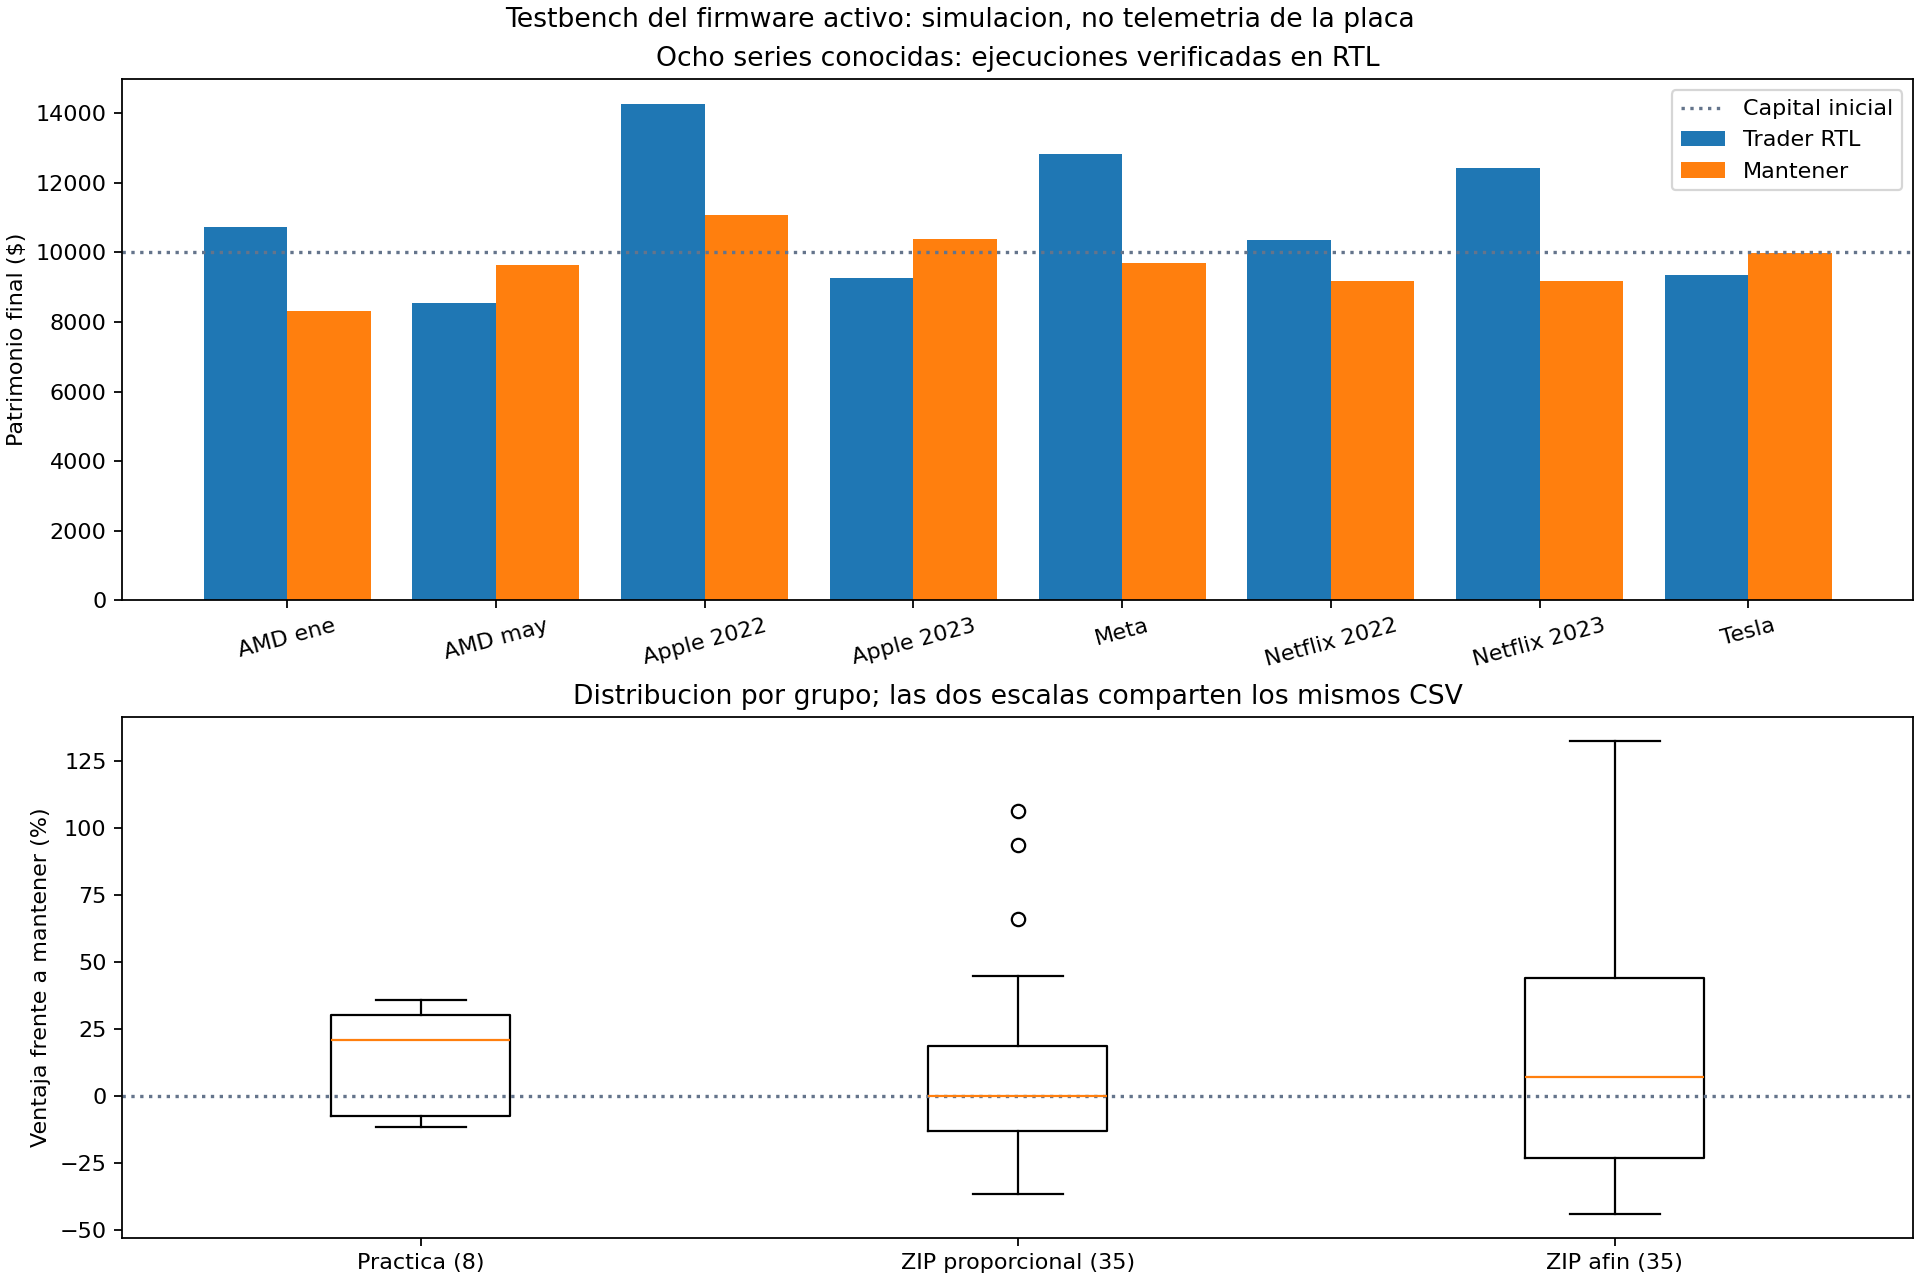
\includegraphics[width=\linewidth]{figuras/todas_acciones_resumen.png}\end{center}
Las dos escalas comparten datos y pueden alterar señales y cantidades.
Sus resultados no deben sumarse como evidencia independiente ni interpretarse
como probabilidad de ganar una ronda secreta. En Netflix 2023 de práctica,
la primera compra se ejecuta en tick 2\,177: a 10 ms implica unos 21,77 segundos
de espera. D4 puede permanecer apagado durante ese intervalo por diseño.

Los 78 CSV RTL se conservan comprimidos en
\path{docs/evidencia_todas_acciones/trazas_rtl/}, con hashes y manifiesto.
\path{tools/auditar_campania_acciones.py} coteja las trazas archivadas con el
modelo sin necesitar el ZIP externo; \path{tools/probar_todas_acciones.py}
repite el ensayo desde los CSV originales. El anexo
\path{resultados_simulacion/testbench_todas_acciones/INFORME_TESTBENCH.pdf}
incluye el detalle y el visor HTML permite filtrar por acción.

\section{Área, timing y rendimiento}
La implementación ocupa \Celdas/1280 LC y \Bram/16 BRAM: quedan 61 LC.
nextpnr informa \Fmax\ MHz en el dominio del SoC. Ese resultado no cambia
su frecuencia configurada de 12,5 MHz. El peor caso observado en las ocho series
es de 259 ciclos, equivalente a 20,72 microsegundos; no es una cota formal
para todas las entradas posibles.

\begin{center}\small\begin{tabular}{lrrrr}\toprule
Serie & Ciclos medios & Ciclos máx. & IC máx. & CPI global \\\midrule
\TablaLatencias\bottomrule\end{tabular}\end{center}
\begin{center}\small\begin{tabular}{lrrr}\toprule
Serie & CPI máximo & Tiempo medio ($\mu$s) & Tiempo máximo ($\mu$s) \\\midrule
\TablaTiempos\bottomrule\end{tabular}\end{center}
Las ventanas miden desde recepción completa del byte hasta DECISION y excluyen
el sondeo posterior. CPI global es ciclos totales divididos por instrucciones
totales; CPI máximo corresponde a un tick individual. Para el período de
100 microsegundos se reservan 9,5 microsegundos de trama y 0,24 de sincronización:
el margen conservador de las series conocidas es $100-9,5-0,24-20,72=69,54$
microsegundos. El estrés RTL de 936 ticks llega a 263 ciclos (21,04 microsegundos):
al incluirlo, el margen conservador observado es 69,22 microsegundos.

\section{Co-diseño hardware/software: estudio histórico}
\label{sec:codisenio}
La auditoría recuperó del commit \texttt{66eede4} el estudio comparativo de
SMA10 anterior a la política final. Se comparan la misma estrategia y la misma
serie de 20\,000 ticks a 25 MHz: software, instrucción \texttt{custom-0} y
periférico MMIO. Son mediciones históricas, no nuevas ejecuciones de la versión
Momentum32. Los CSV resumidos, informe original y manifiesto de procedencia
están en \path{docs/evidencia_codisenio/}; los programas, RTL, testbenches y
trazas completas se conservan en ese commit del repositorio.

\subsection{Kernel, alternativas y recursos}
El perfil original identifica 163,93 ciclos medios en SMA10. El kernel ampliado
de historial, SMA y señal ocupa 186,62 de 218,66 ciclos/tick. La instrucción
\texttt{smaupd} fusiona la actualización $rd\leftarrow rd-rs1+rs2$ y añade un
tercer puerto de lectura de registros. El periférico MMIO conserva diez precios
y actualiza la suma al recibir cada byte; Espino sigue decidiendo la operación.

\begin{center}\small\begin{tabular}{lrrrrrr}\toprule
Variante & LUT4 & LC/1280 & BRAM/16 & Fmax (MHz) & Ciclos medios & CPI \\\midrule
Software & 980 & 1200 & 12 & 42,60 & 218,66 & 2,379 \\
custom-0 & 1133 & 1350 & 14 & No enruta & 70,73 & 2,286 \\
MMIO SMA10 & 1055 & 1279 & 13 & 40,50 & 60,64 & 2,259 \\\bottomrule
\end{tabular}\end{center}
Las LC combinan funciones de LUT y registro; se presentan separadas de LUT4.
\texttt{custom-0} excede el dispositivo por 70 LC: no tiene Fmax válida de
enrutado ni se considera una opción programable en HX1K. MMIO sí cabe, pero
el diseño de aquella etapa dejaba solo una LC libre.

\subsection{Ops/s y ley de Amdahl}
Aquí una operación útil es procesar un tick y escribir DECISION. La capacidad
del core es $25\cdot10^6/C$ ticks/s, con $C$ ciclos medios por tick. El estímulo
histórico llegaba cada 30 microsegundos, limitando el caudal a 33\,333 ticks/s.
Capacidad de servicio y caudal de entrada son magnitudes distintas.

\begin{center}\small\begin{tabular}{lrrrrr}\toprule
Variante & IC medios & Ciclos máx. & Capacidad (ticks/s) & Speedup & Amdahl \\\midrule
Software & 91,92 & 412 & 114\,331 & 1,000 & 1,000 \\
custom-0 & 30,94 & 266 & 353\,435 & 3,091 & 3,076 \\
MMIO SMA10 & 26,85 & 255 & 412\,270 & 3,606 & 3,692 \\\bottomrule
\end{tabular}\end{center}
Se usa $P=186,62425/218,6635\simeq0,8535$ y
\[
S_{\mathrm{Amdahl}}=\frac{1}{(1-P)+P/S_k},\qquad
S_k=\frac{186,62425}{C_{k,\mathrm{variante}}}.
\]
Los kernels medidos de custom-0 y MMIO son 39,04 y 27,18 ciclos, respectivamente.
Su perfil regional usa 100 ticks; los tiempos totales y el speedup observado
usan 20\,000. Esa diferencia de muestra y el trabajo fuera del kernel explican
que la predicción no coincida exactamente con el speedup total.

\subsection{Roofline simplificado y decisión final}
Para el roofline, operación significa suma/resta entera, no tick. El modelo
supone pico de 25 Mops/s, ancho de banda de BRAM de 50 MB/s y
$P(I)=\min(25,50I)$ Mops/s. Se excluyen tráfico de instrucciones, polling y
control; el ancho de banda es un supuesto de arquitectura, no una medición.

\begin{center}\small\begin{tabular}{lrrrr}\toprule
Kernel & Operaciones & Bytes/tick & Intensidad (ops/B) & Techo (Mops/s) \\\midrule
Software & 14 & 41 & 0,341 & 17,07 \\
custom-0 & 6 & 5 & 1,200 & 25,00 \\
MMIO SMA10 & 6 & 11 & 0,545 & 25,00 \\\bottomrule
\end{tabular}\end{center}
\begin{center}
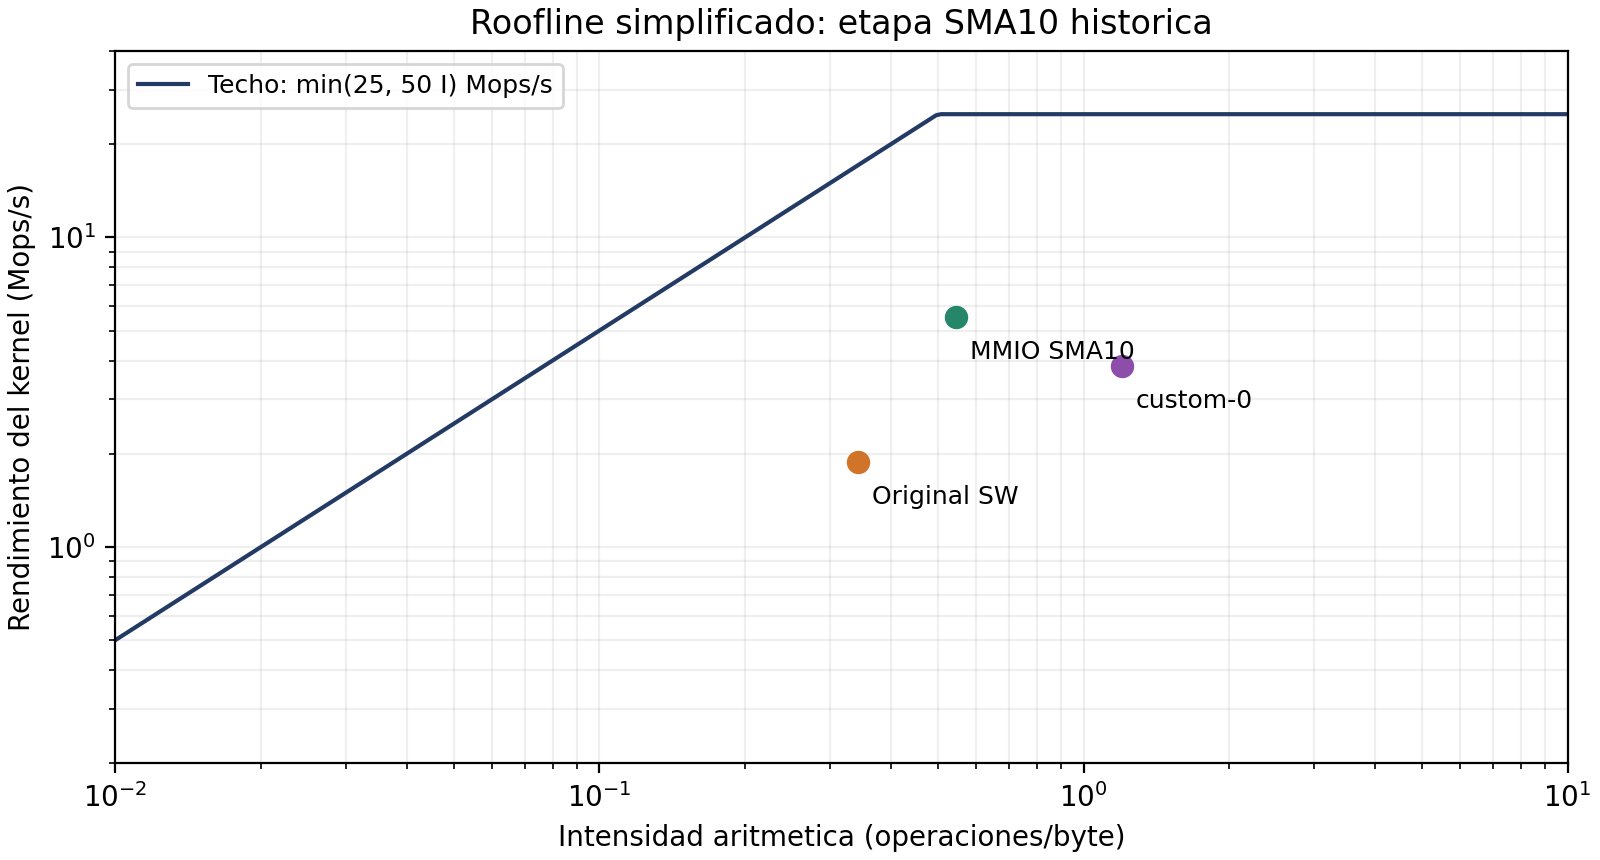
\includegraphics[width=0.88\linewidth]{figuras/roofline_historico.png}
\end{center}
Los puntos combinan los conteos aproximados declarados y la latencia regional
medida; no son pruebas de ancho de banda ni una caracterización del firmware
final. El kernel software queda bajo el techo de memoria del modelo, mientras
las dos alternativas se ubican bajo el techo de cómputo.

El estudio justifica descartar custom-0 por área y conservar MMIO como opción
implementable. La integración final cambia la política a Momentum32 con stop
y reduce el reloj del SoC a 12,5 MHz para usar el arranque validado. SUM10 sigue
presente, pero no participa en la regla final: no corresponde atribuirle un
speedup de 3,606 a Momentum32. Su evaluación propia está en la sección de
latencia y ocupa \Celdas\ LC y \Bram\ BRAM. Falta un perfil regional y una
comparación de variantes bajo la misma política final para cerrar esa extensión
del estudio sin mezclar mejoras de algoritmo y mejoras de hardware.


\section{Programación, reproducción y auditoría}
La imagen activa tiene las siguientes firmas:
\begin{flushleft}\small BIN: \texttt{\BinSHA}\\
HEX: \texttt{\HexSHA}\end{flushleft}
Desde la raíz del proyecto se verifica y programa manualmente:
\begin{lstlisting}
python -B tools/trader.py verify
iceprog competition.bin
iceprog -c competition.bin
python simular_competencia.py
\end{lstlisting}
\texttt{programar.ps1 -SoloVerificar} comprueba archivos sin escribir la placa.
El build no ejecuta iceprog. El visor reproduce el modelo precalculado, cotejado
con trazas RTL cuando están disponibles; no recibe telemetría de la Go Board.
\path{COMO_SIMULAR.md} incluye los comandos de testbench y exportación.

La imagen anterior con hash iniciado en \texttt{5e1579ca} está respaldada en
\path{respaldos/momentum32_fisico_5e1579ca/}; su registro de dos
\texttt{VERIFY OK} y compras/ventas corresponde a aquella sesión.
El grupo confirmó posteriormente la reprogramación de la imagen lenta.
La declaración y su asociación con el BIN local se registran en
\path{docs/evidencia_fisica/reprogramacion_tendencia_lenta.json}.
La campaña ampliada utiliza su mismo firmware y RTL; sus cifras son resultados
de simulación y no una lectura de la flash ni una traza física de la maestra.
Quedan por documentar los resultados oficiales de las tres rondas, la
acreditación de defensa y el perfil regional del kernel de la política lenta.
La auditoría separada conserva estos pendientes; no asigna una nota.

\section{Conclusiones}
Se integró la tendencia lenta original en Espino RV32E conservando la corrección
de recepción SPI y la contabilidad causal de la competencia. La igualdad de
160\,000 ticks entre modelo, intérprete de instrucciones y RTL respalda que el comportamiento
implementado coincide con la política descrita. La campaña ampliada verifica
además 1\,557\,620 ticks del RTL activo en 78 escenarios sin discrepancias,
incluyendo 428 compras y 364 ventas. La síntesis cabe en HX1K y el
peor tiempo observado de 21,04 microsegundos deja margen para la ronda de 100 microsegundos. La
reconstrucción del BIN verifica que también la imagen empaquetada responde con
compras y ventas en el escenario de integración.

Esta integración cambia de forma importante lo que se observará: la placa
comienza en caja y puede esperar cientos de ticks o permanecer sin operar si
las revisiones no superan el 5\%. Una subida lenta acumulada no garantiza entrada,
pues el ancla se renueva cada 128 ticks. Esta propiedad explica parte de la
protección y también las oportunidades perdidas. No conviene diagnosticar una
falla únicamente por ausencia de D4; deben revisarse recepción, lectura y serie.

Financieramente, la nueva versión mejora algunos casos y reduce el máximo
drawdown observado, pero pierde patrimonio medio frente a Momentum32 con stop.
El resultado 5/8 frente a mantener y las pérdidas de AMD mayo, Apple 2023 y
Tesla impiden sostener que siempre es mejor. Su elección es una decisión del
grupo con un compromiso entre respuesta, exposición y riesgo, no una garantía
de ganar las tres rondas. Los adicionales refuerzan esa cautela: 16/35 ventajas
en proporcional y 18/35 en afín, con pérdidas y períodos sin operar. La mejora
de algunos casos convive con oportunidades perdidas y depende de la escala.
Se conserva la versión anterior como referencia reproducible.

El grupo reportó la reprogramación de la placa y la validación digital está
completa para los escenarios declarados. Para cerrar la entrega deben adjuntarse
los registros de competencia y defensa. El estudio histórico de Amdahl y roofline
aporta contexto de co-diseño, pero no reemplaza una comparación de alternativas
con la política lenta. Mantener separados esos alcances hace que el informe
sea reproducible y que sus conclusiones respondan a lo realmente comprobado.

\appendix\clearpage\section{Gráficos de las ocho series}
Misma política y contabilidad en todos los casos. Los marcadores son ejecuciones.
\clearpage\subsection{AMD enero 2022}
\begin{center}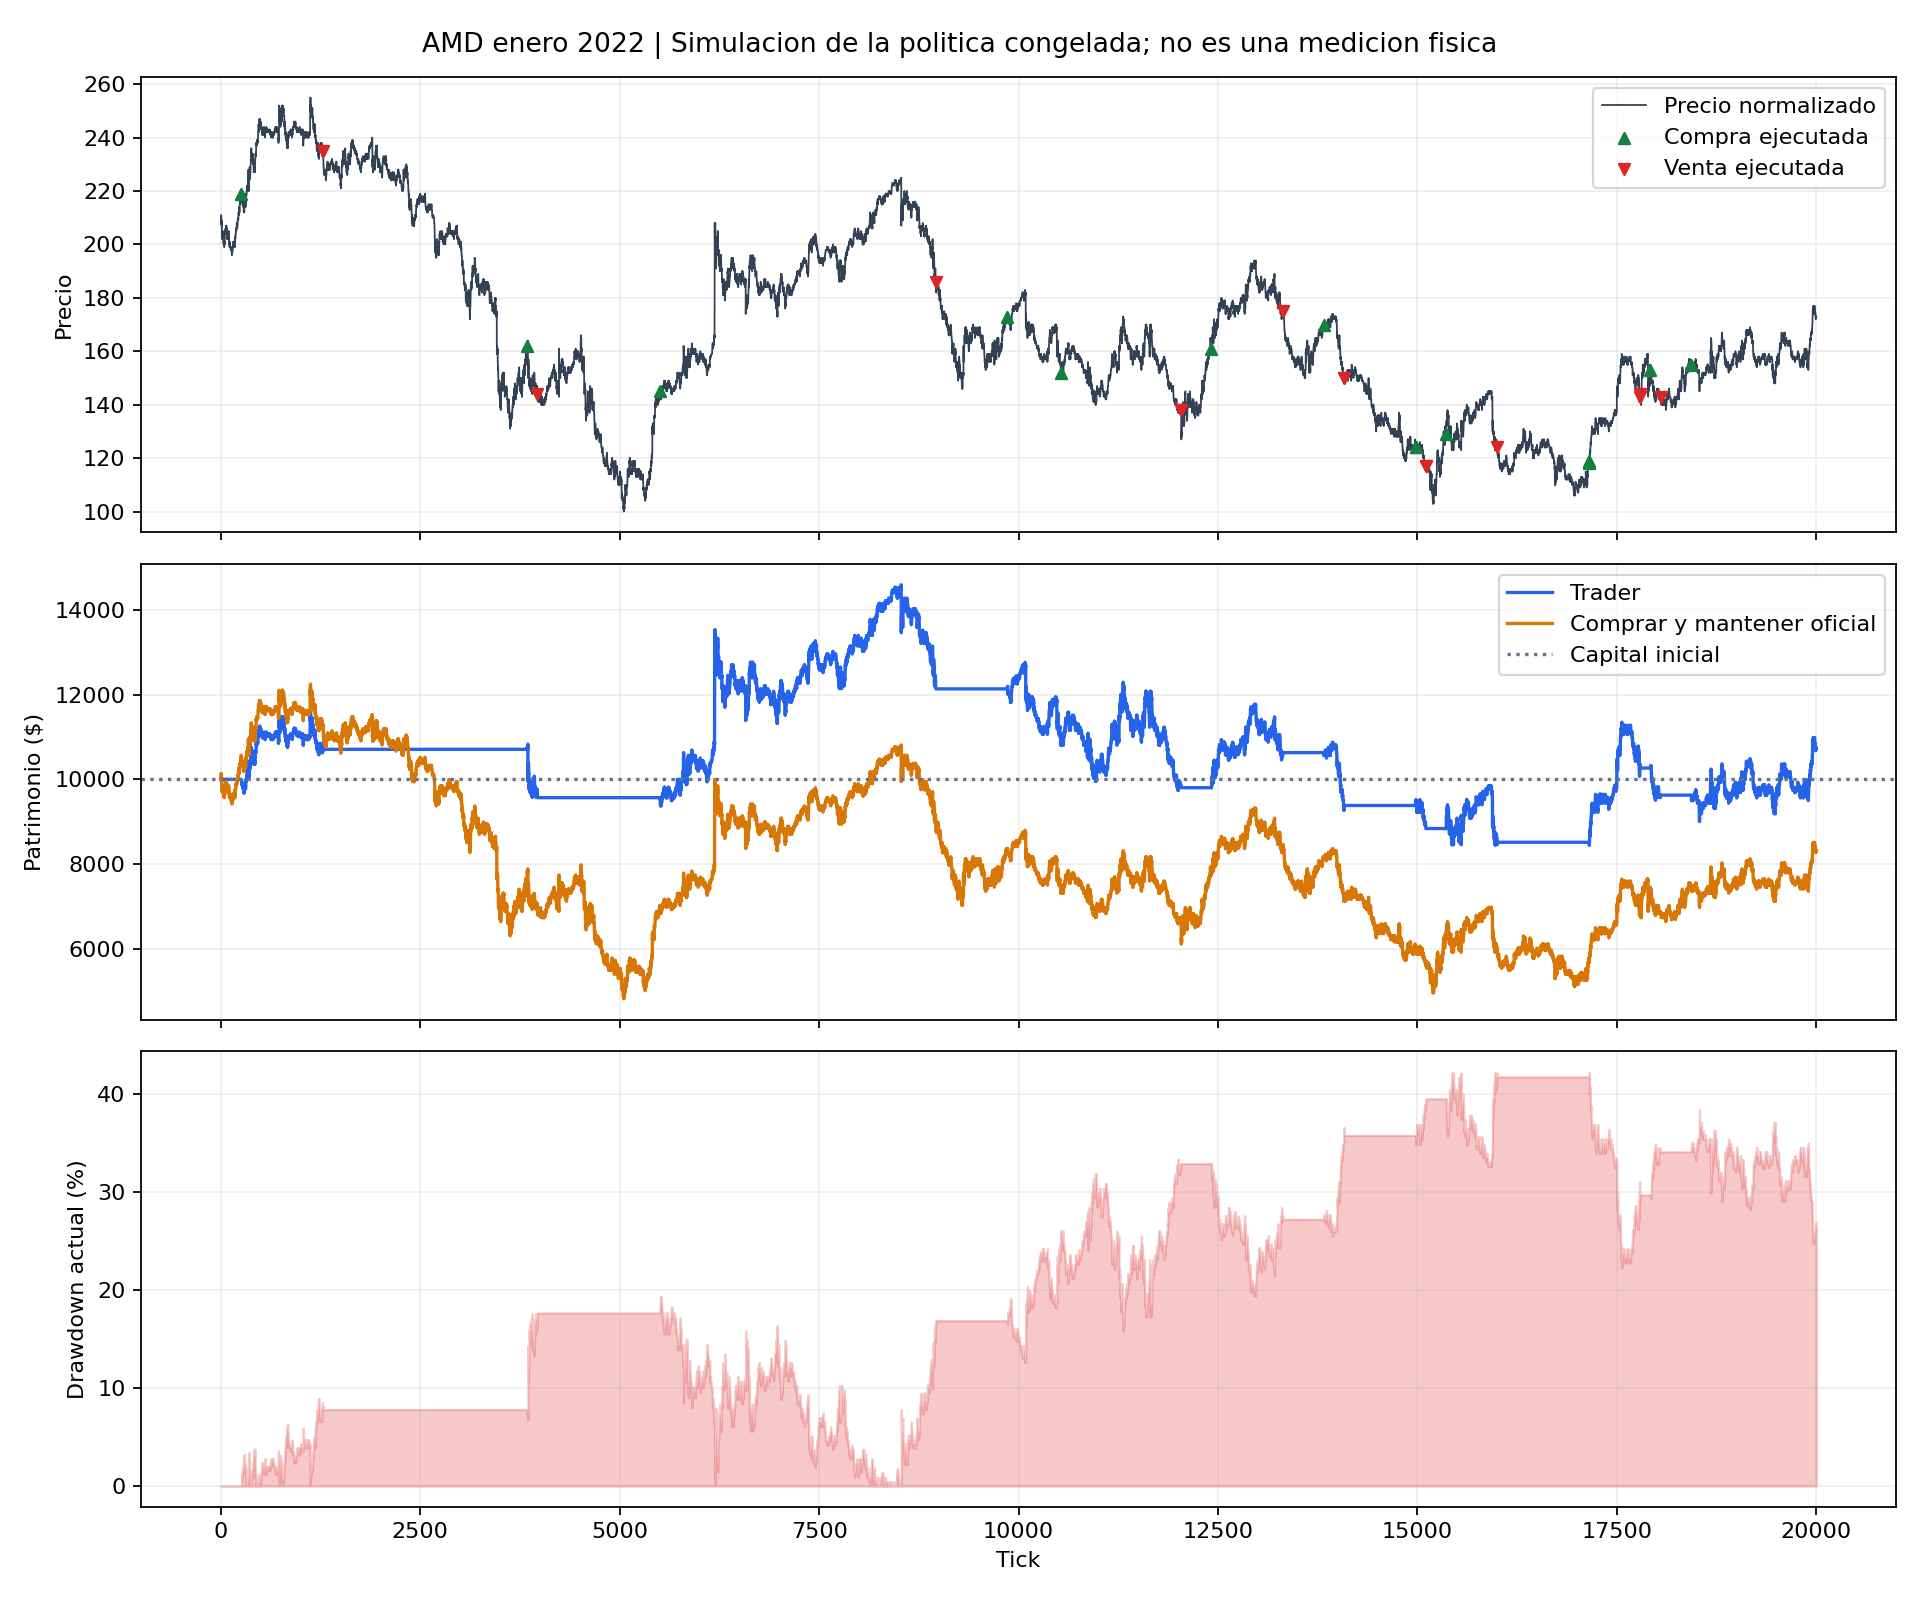
\includegraphics[width=\linewidth,height=0.70\textheight,keepaspectratio]{figuras/amd_enero.png}\end{center}
Trader: \$10\,738; mantener: \$8\,315; ventaja: \$2\,423. Órdenes: 27; comisiones: \$135; drawdown máximo: 42,20\%.

Los marcadores representan ejecuciones al precio siguiente al que generó la señal. Es simulación sobre datos conocidos; no es telemetría de la placa.

\clearpage\subsection{AMD mayo 2022}
\begin{center}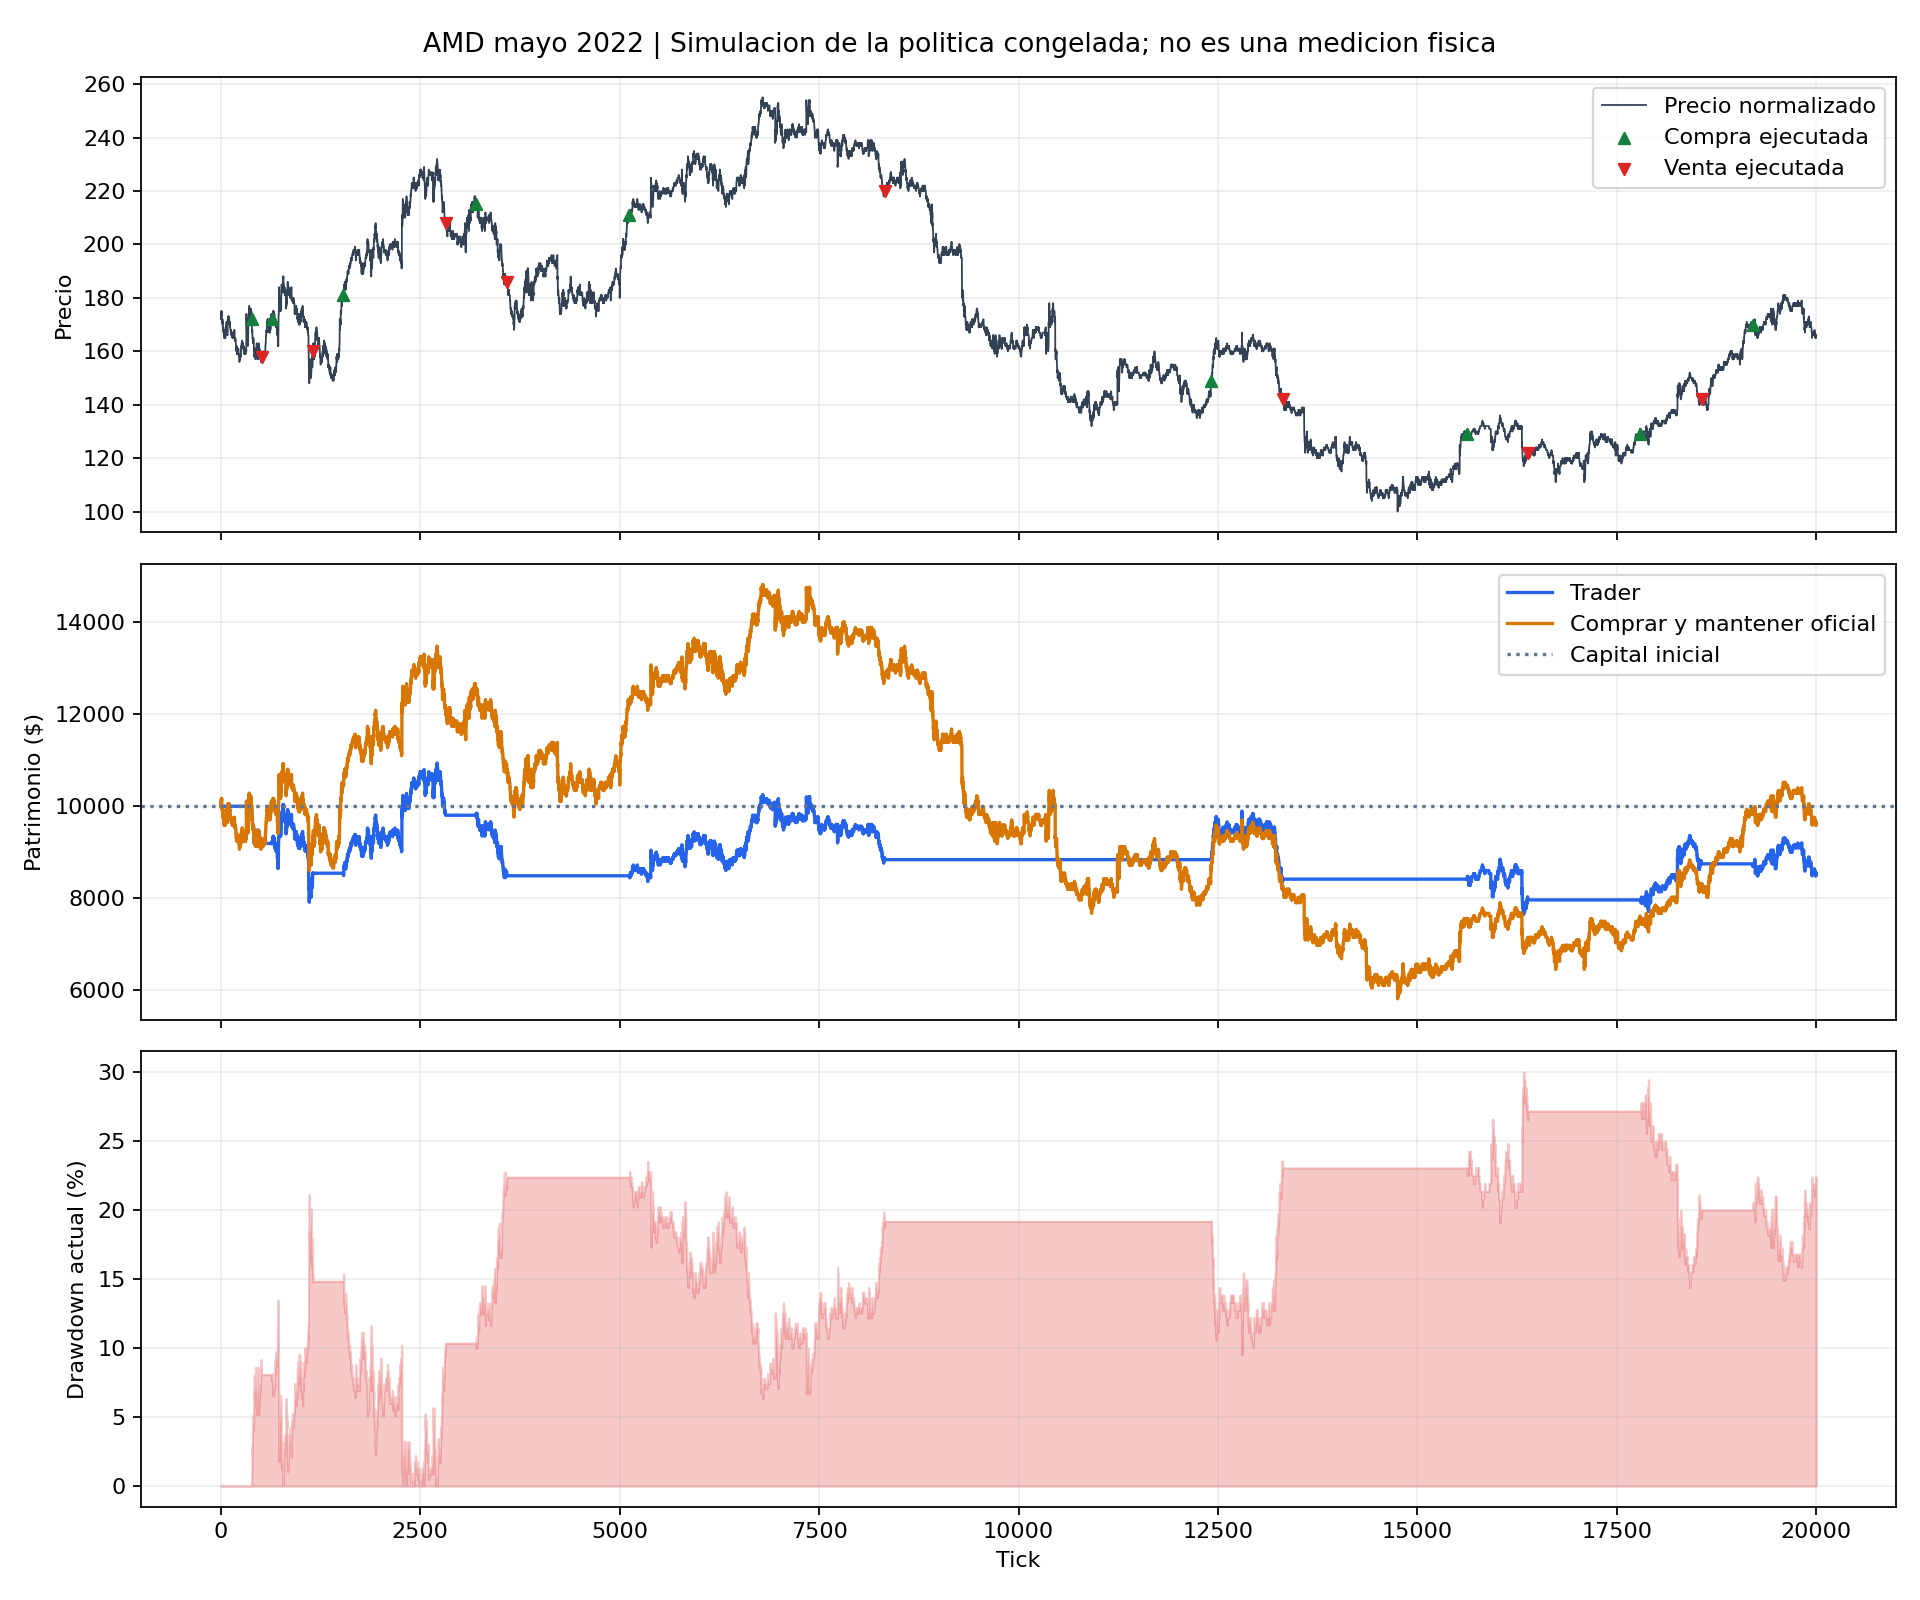
\includegraphics[width=\linewidth,height=0.70\textheight,keepaspectratio]{figuras/amd_mayo.png}\end{center}
Trader: \$8\,540; mantener: \$9\,647; ventaja: \$-1\,107. Órdenes: 17; comisiones: \$85; drawdown máximo: 30,01\%.

Los marcadores representan ejecuciones al precio siguiente al que generó la señal. Es simulación sobre datos conocidos; no es telemetría de la placa.

\clearpage\subsection{Apple 2022}
\begin{center}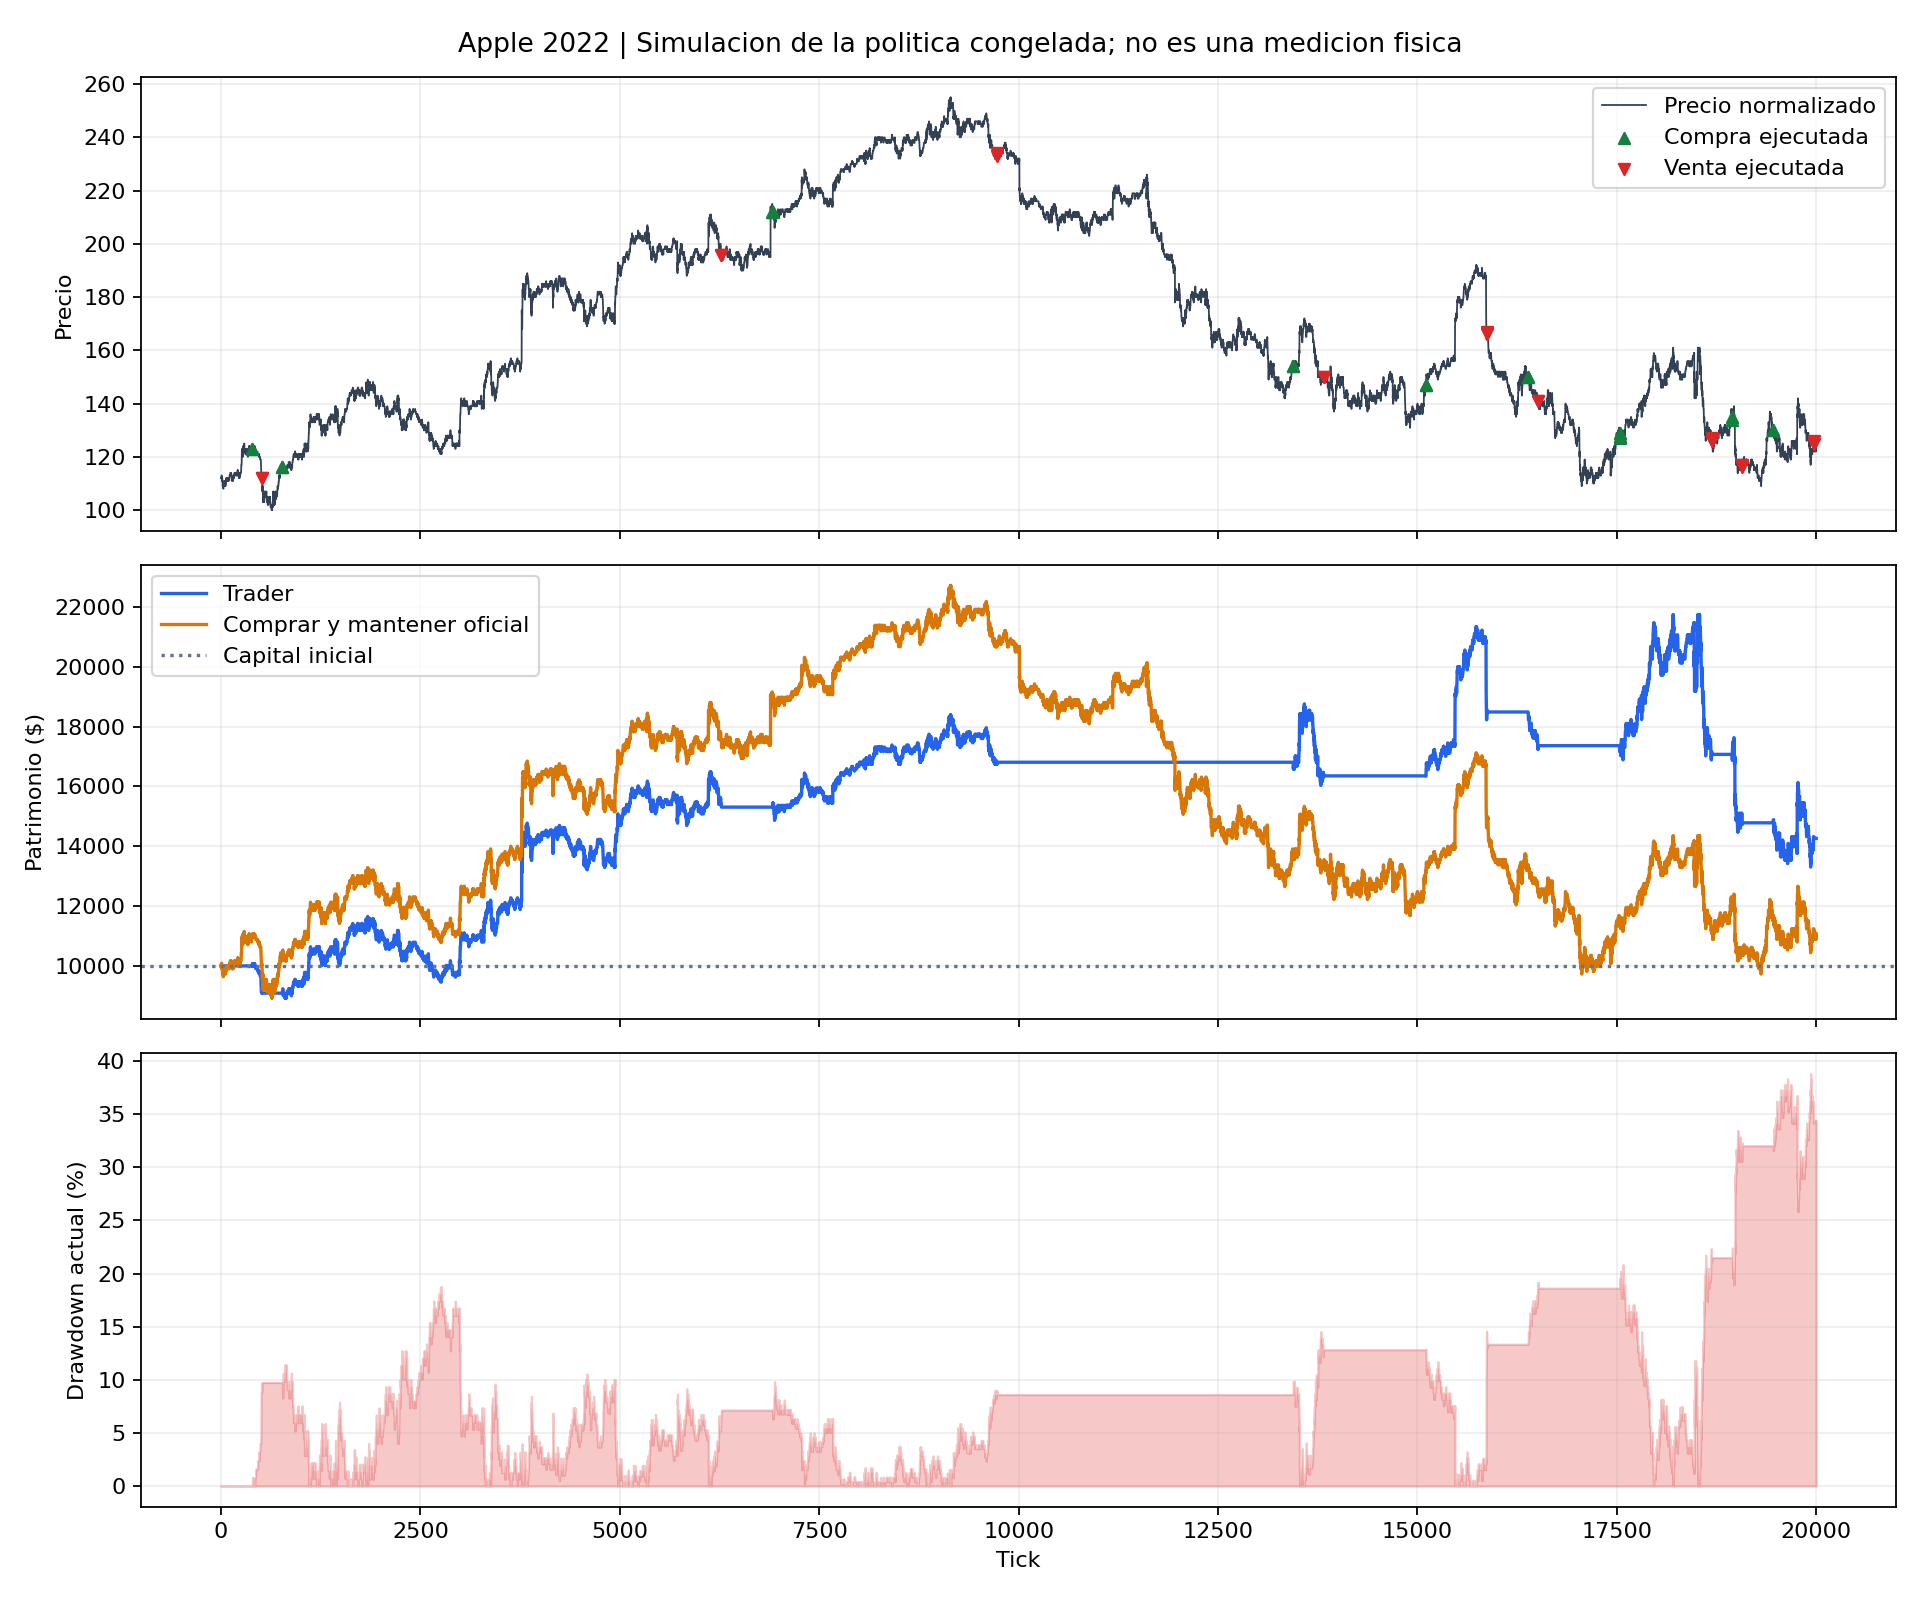
\includegraphics[width=\linewidth,height=0.70\textheight,keepaspectratio]{figuras/apple_2022.png}\end{center}
Trader: \$14\,263; mantener: \$11\,063; ventaja: \$3\,200. Órdenes: 38; comisiones: \$190; drawdown máximo: 38,82\%.

Los marcadores representan ejecuciones al precio siguiente al que generó la señal. Es simulación sobre datos conocidos; no es telemetría de la placa.

\clearpage\subsection{Apple 2023}
\begin{center}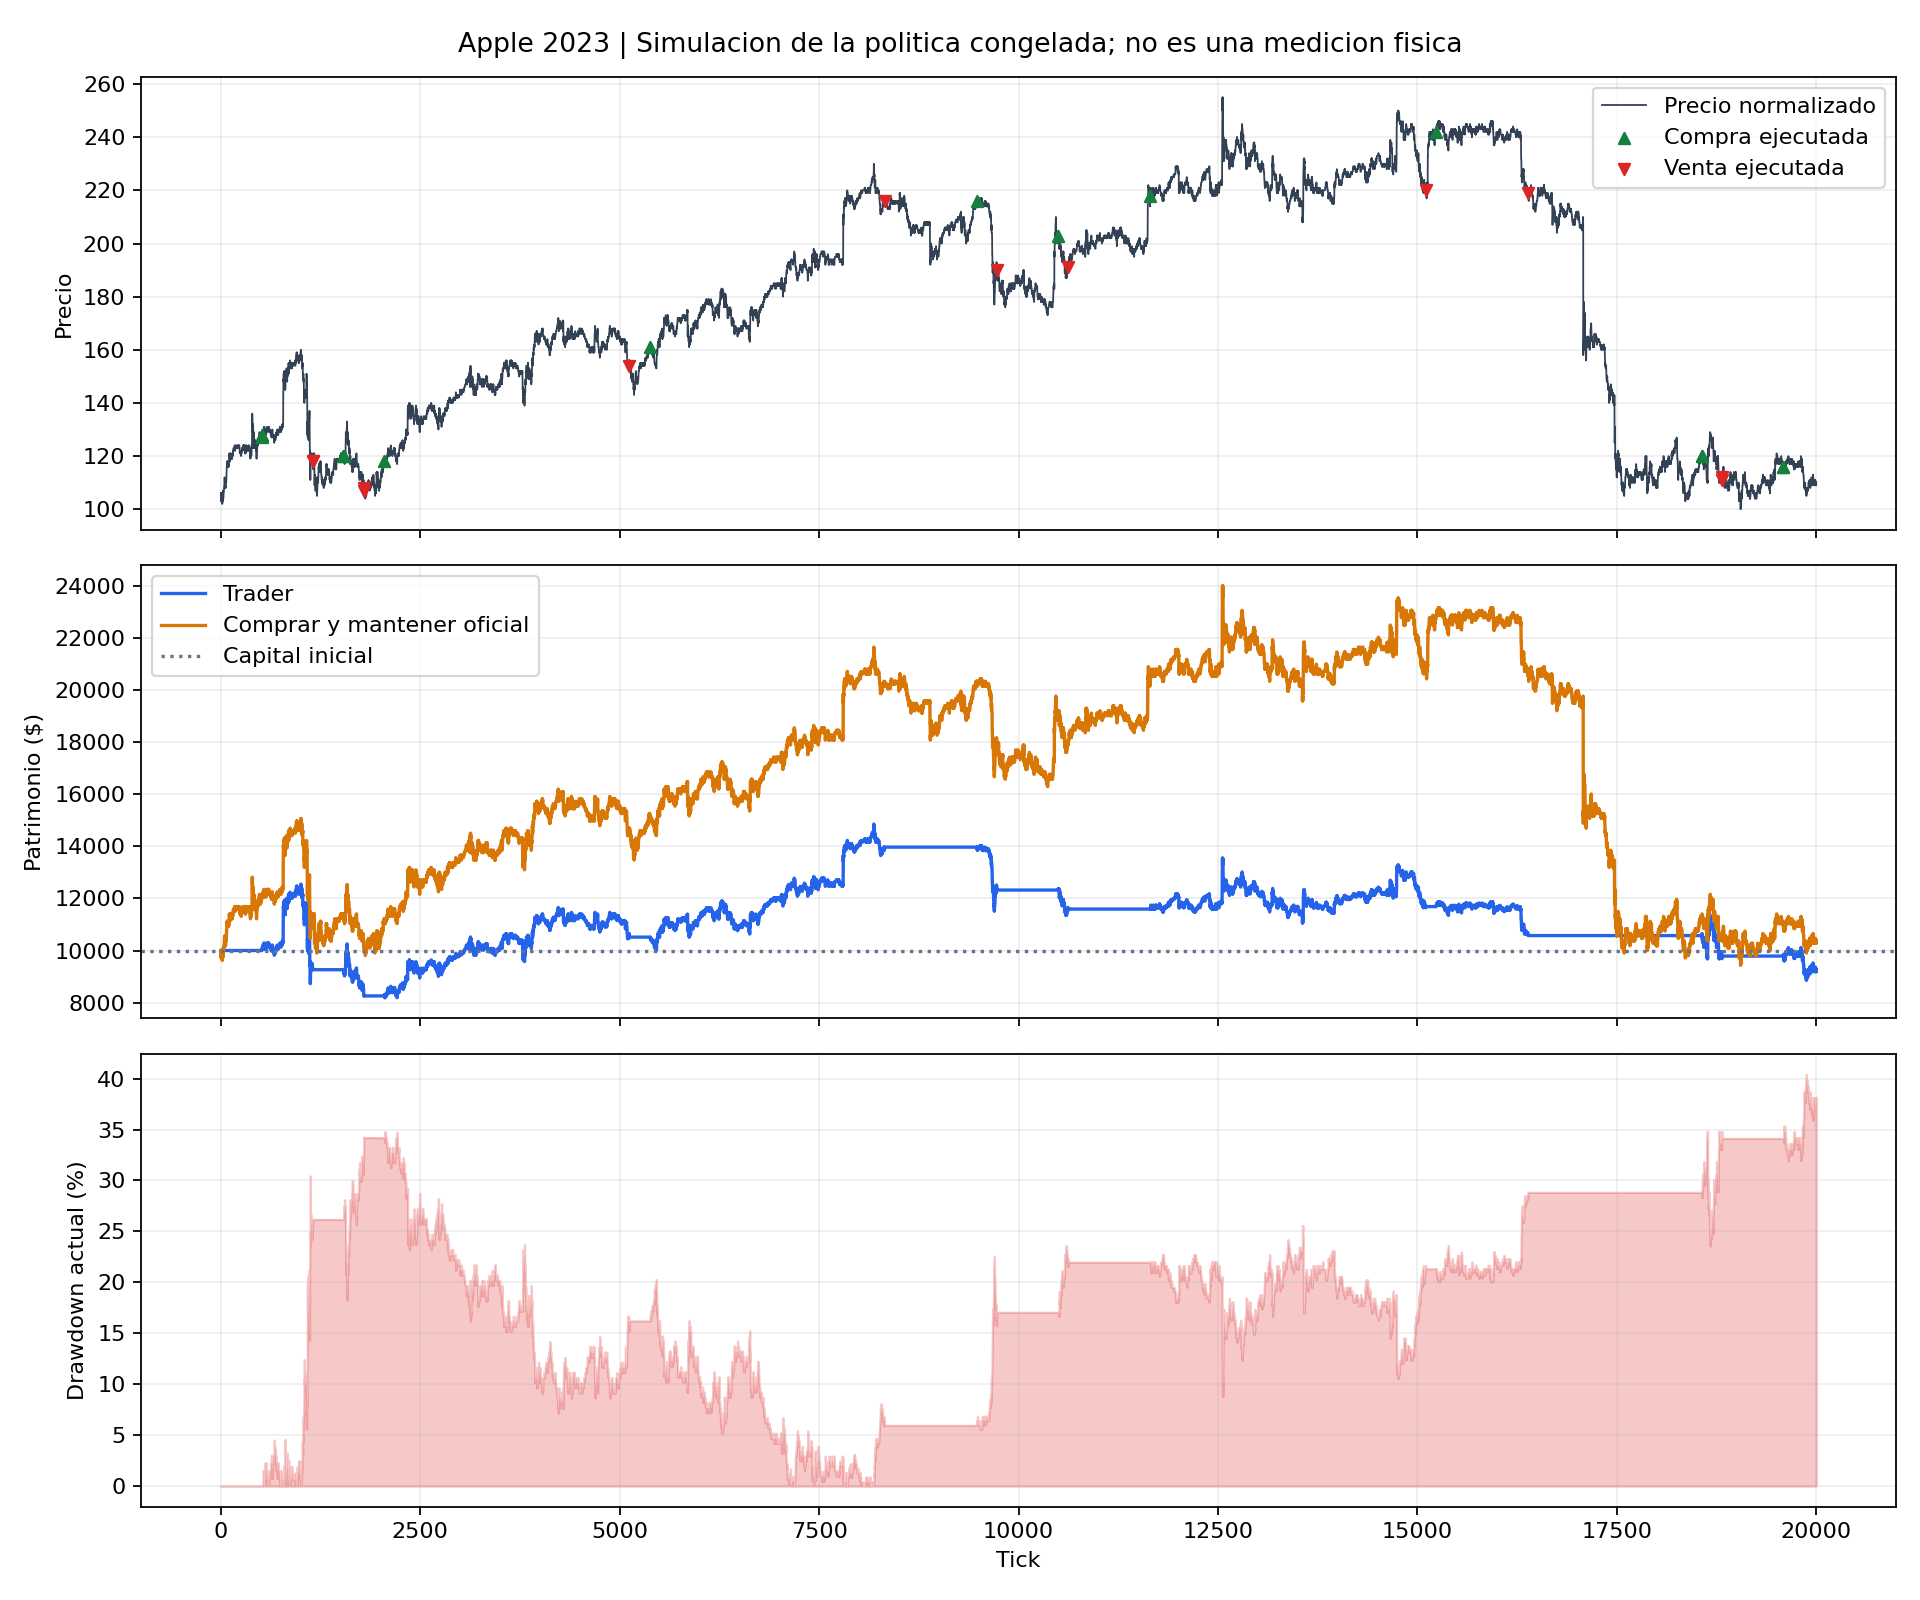
\includegraphics[width=\linewidth,height=0.70\textheight,keepaspectratio]{figuras/apple_2023.png}\end{center}
Trader: \$9\,272; mantener: \$10\,371; ventaja: \$-1\,099. Órdenes: 26; comisiones: \$130; drawdown máximo: 40,41\%.

Los marcadores representan ejecuciones al precio siguiente al que generó la señal. Es simulación sobre datos conocidos; no es telemetría de la placa.

\clearpage\subsection{Meta 2022}
\begin{center}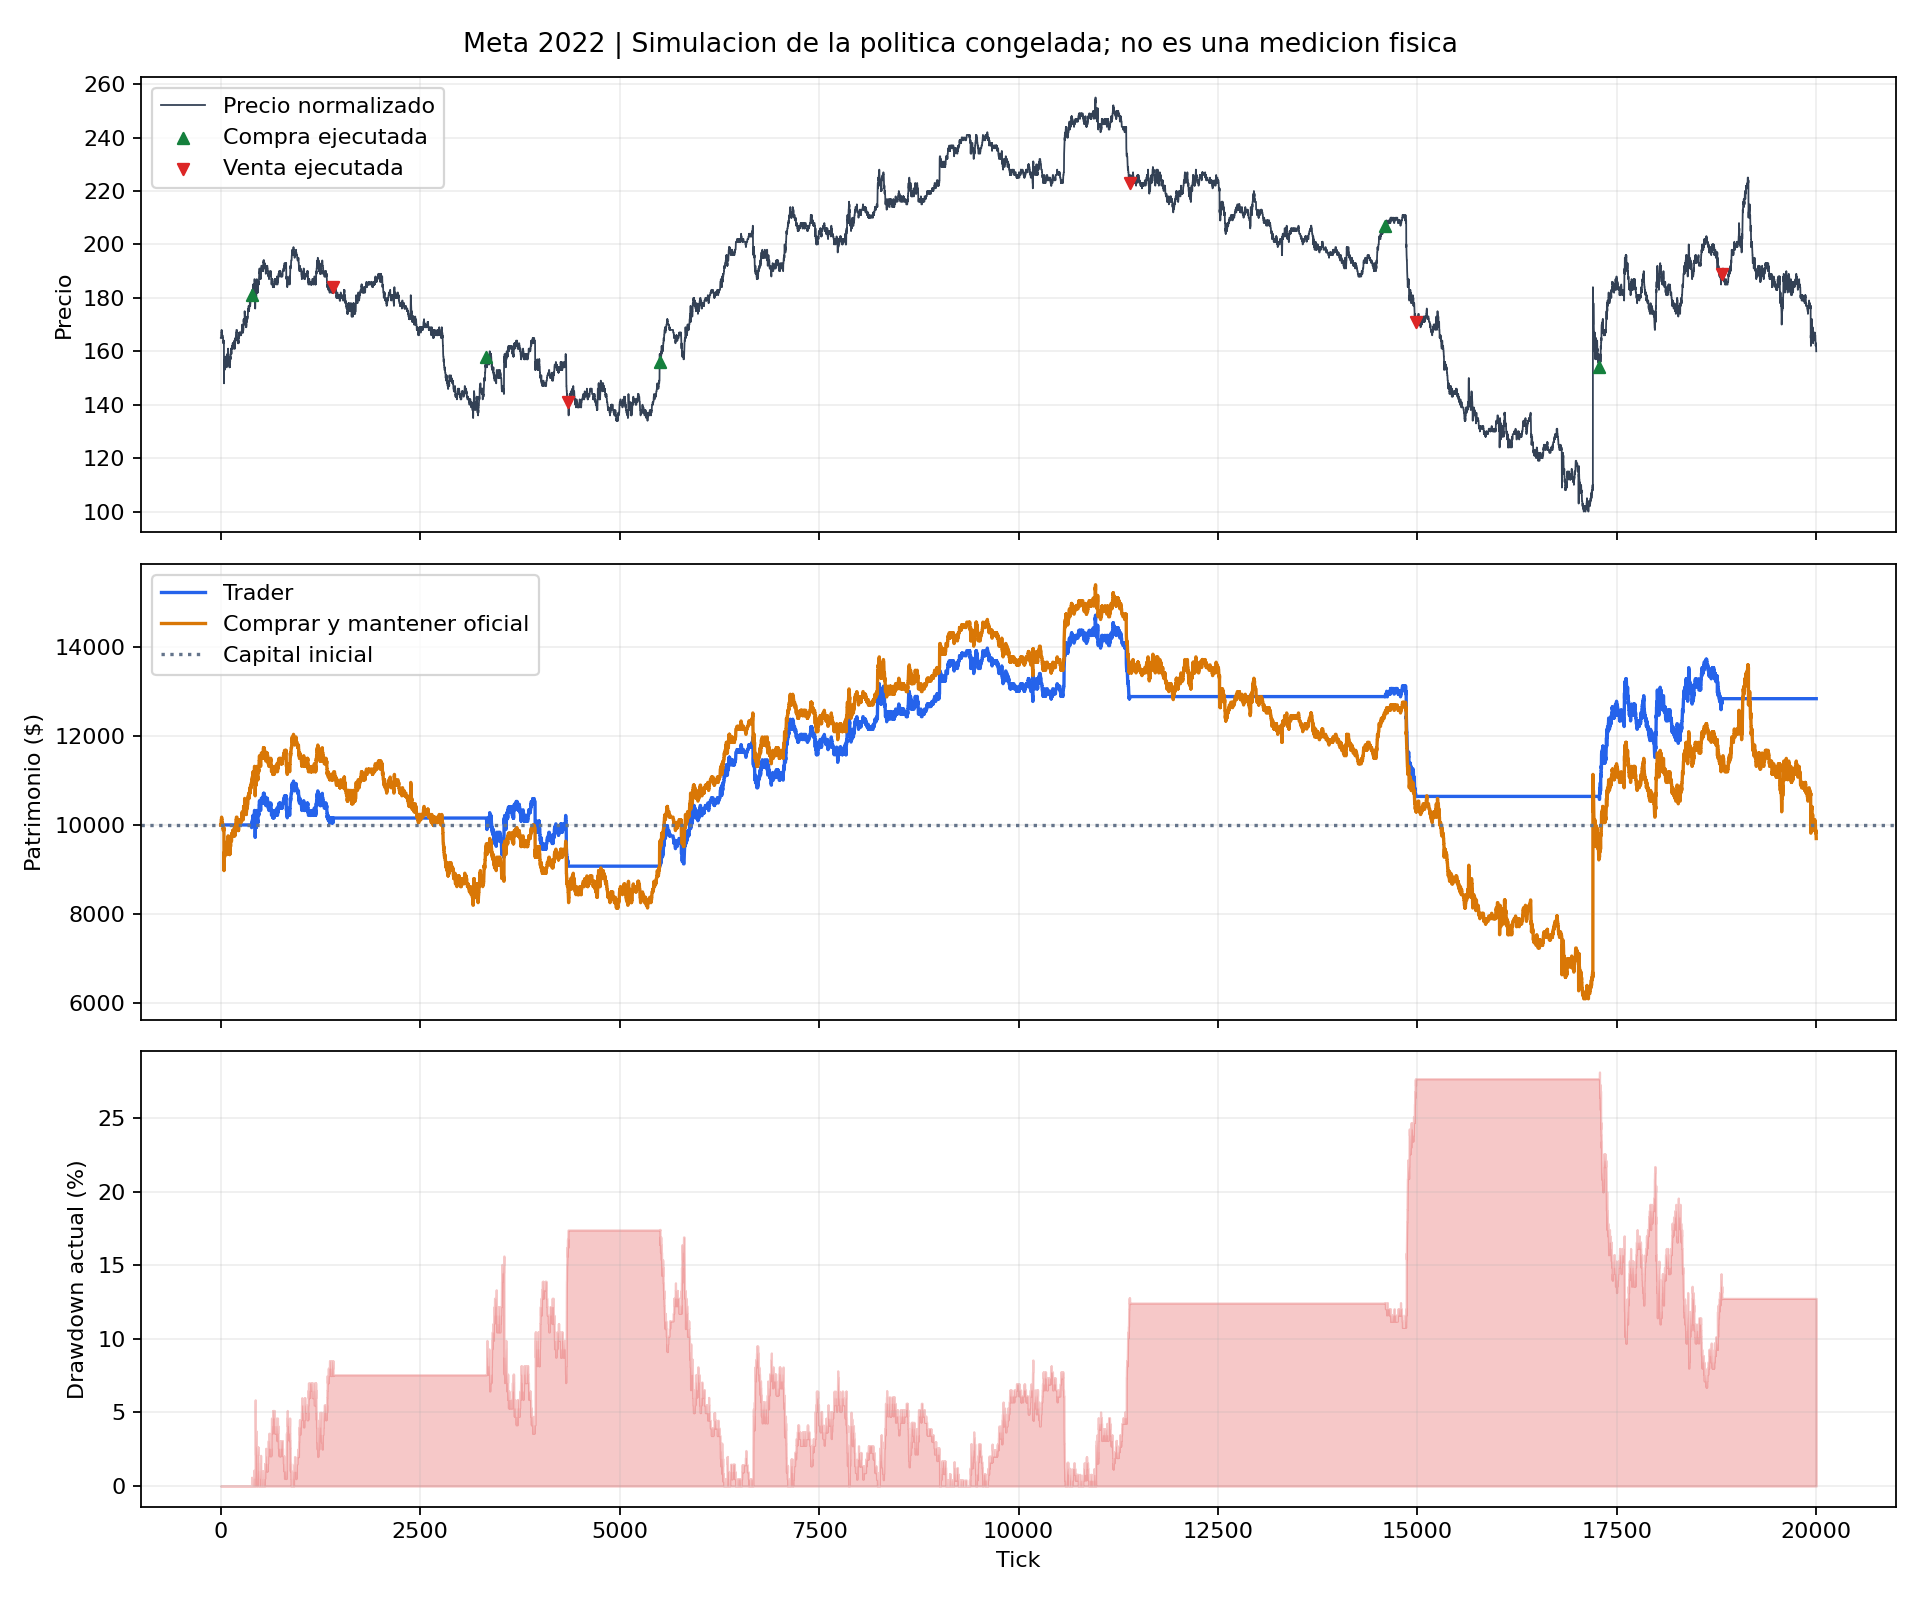
\includegraphics[width=\linewidth,height=0.70\textheight,keepaspectratio]{figuras/meta_2022.png}\end{center}
Trader: \$12\,836; mantener: \$9\,695; ventaja: \$3\,141. Órdenes: 10; comisiones: \$50; drawdown máximo: 28,13\%.

Los marcadores representan ejecuciones al precio siguiente al que generó la señal. Es simulación sobre datos conocidos; no es telemetría de la placa.

\clearpage\subsection{Netflix 2022}
\begin{center}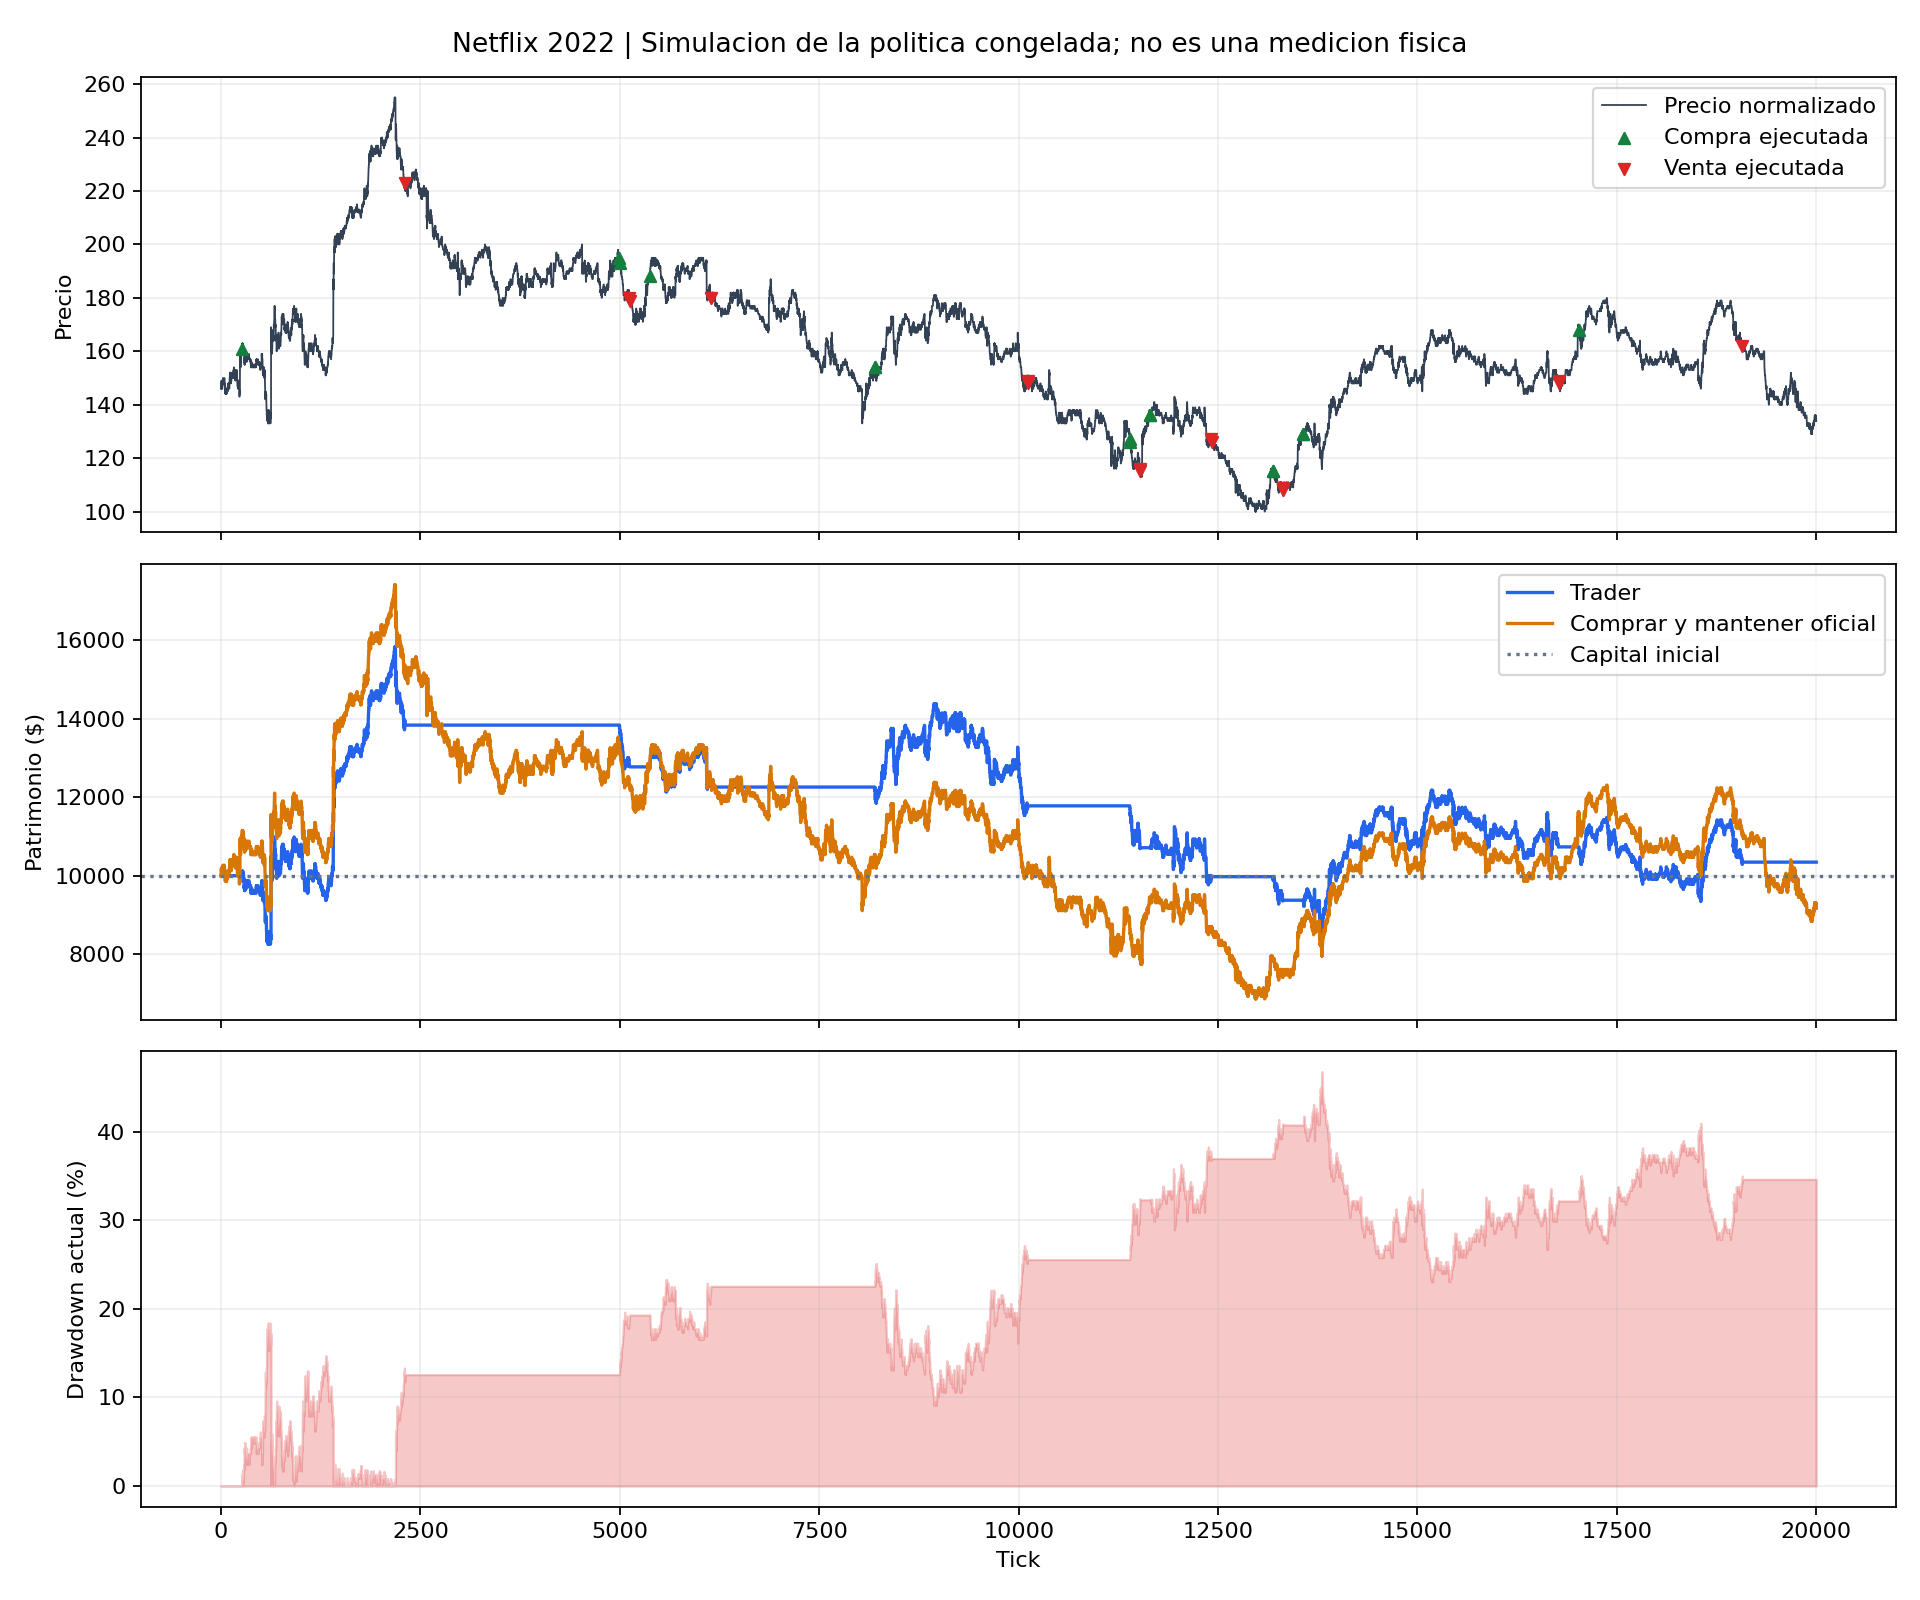
\includegraphics[width=\linewidth,height=0.70\textheight,keepaspectratio]{figuras/netflix_2022.png}\end{center}
Trader: \$10\,346; mantener: \$9\,179; ventaja: \$1\,167. Órdenes: 30; comisiones: \$150; drawdown máximo: 46,72\%.

Los marcadores representan ejecuciones al precio siguiente al que generó la señal. Es simulación sobre datos conocidos; no es telemetría de la placa.

\clearpage\subsection{Netflix 2023}
\begin{center}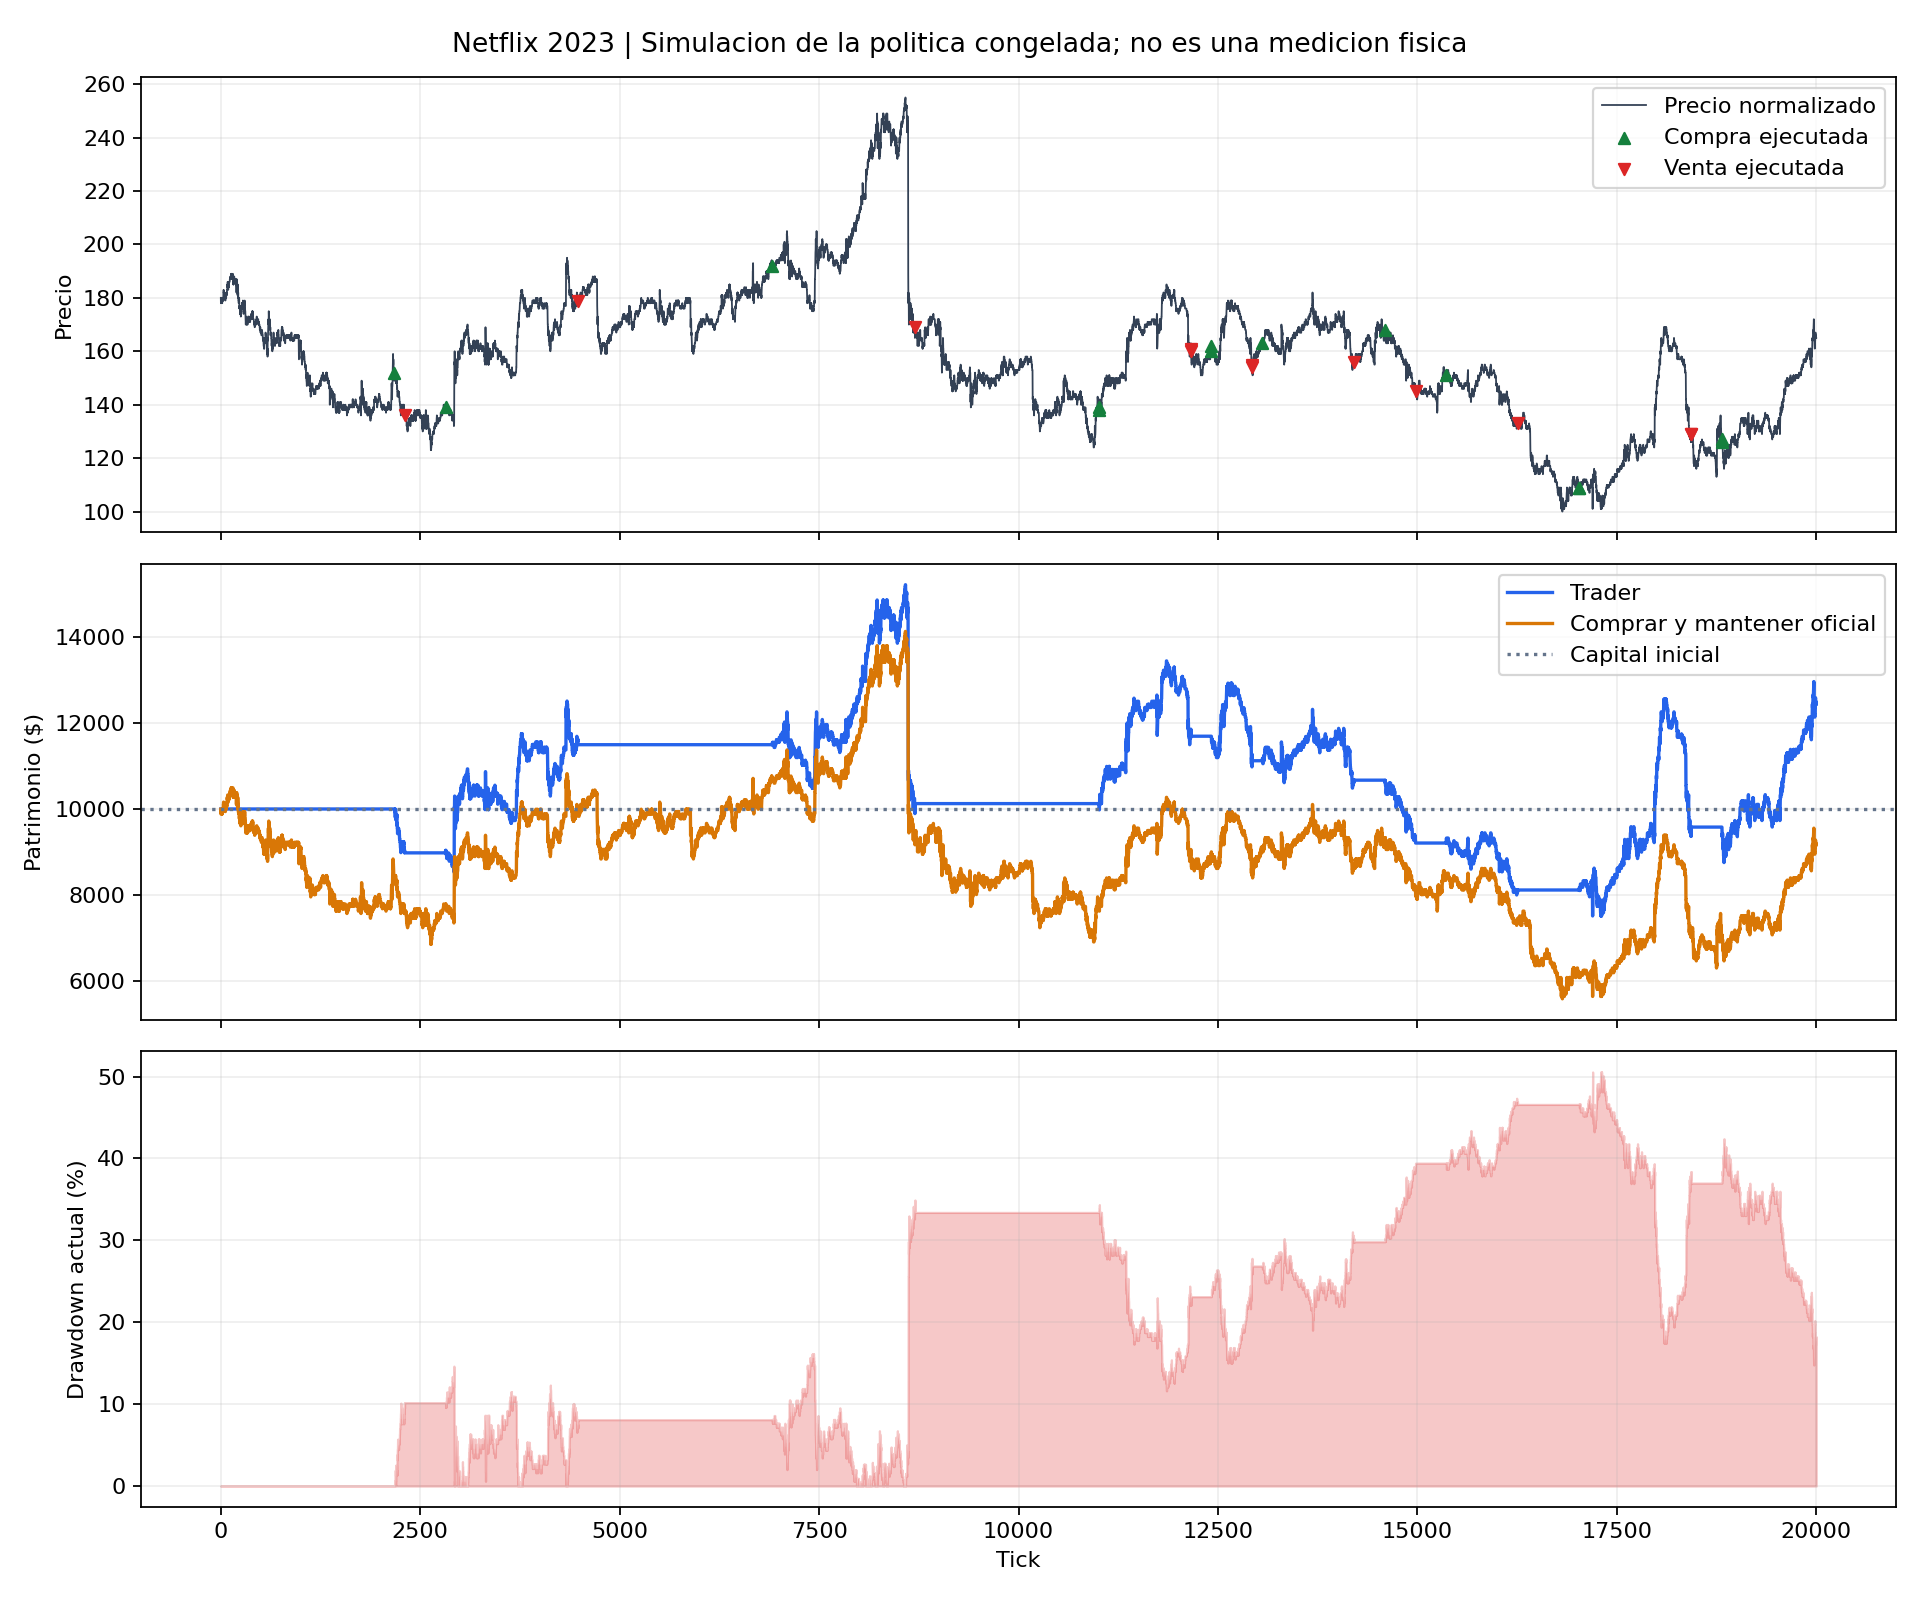
\includegraphics[width=\linewidth,height=0.70\textheight,keepaspectratio]{figuras/netflix_2023.png}\end{center}
Trader: \$12\,432; mantener: \$9\,170; ventaja: \$3\,262. Órdenes: 26; comisiones: \$130; drawdown máximo: 50,55\%.

Los marcadores representan ejecuciones al precio siguiente al que generó la señal. Es simulación sobre datos conocidos; no es telemetría de la placa.

\clearpage\subsection{Tesla 2022}
\begin{center}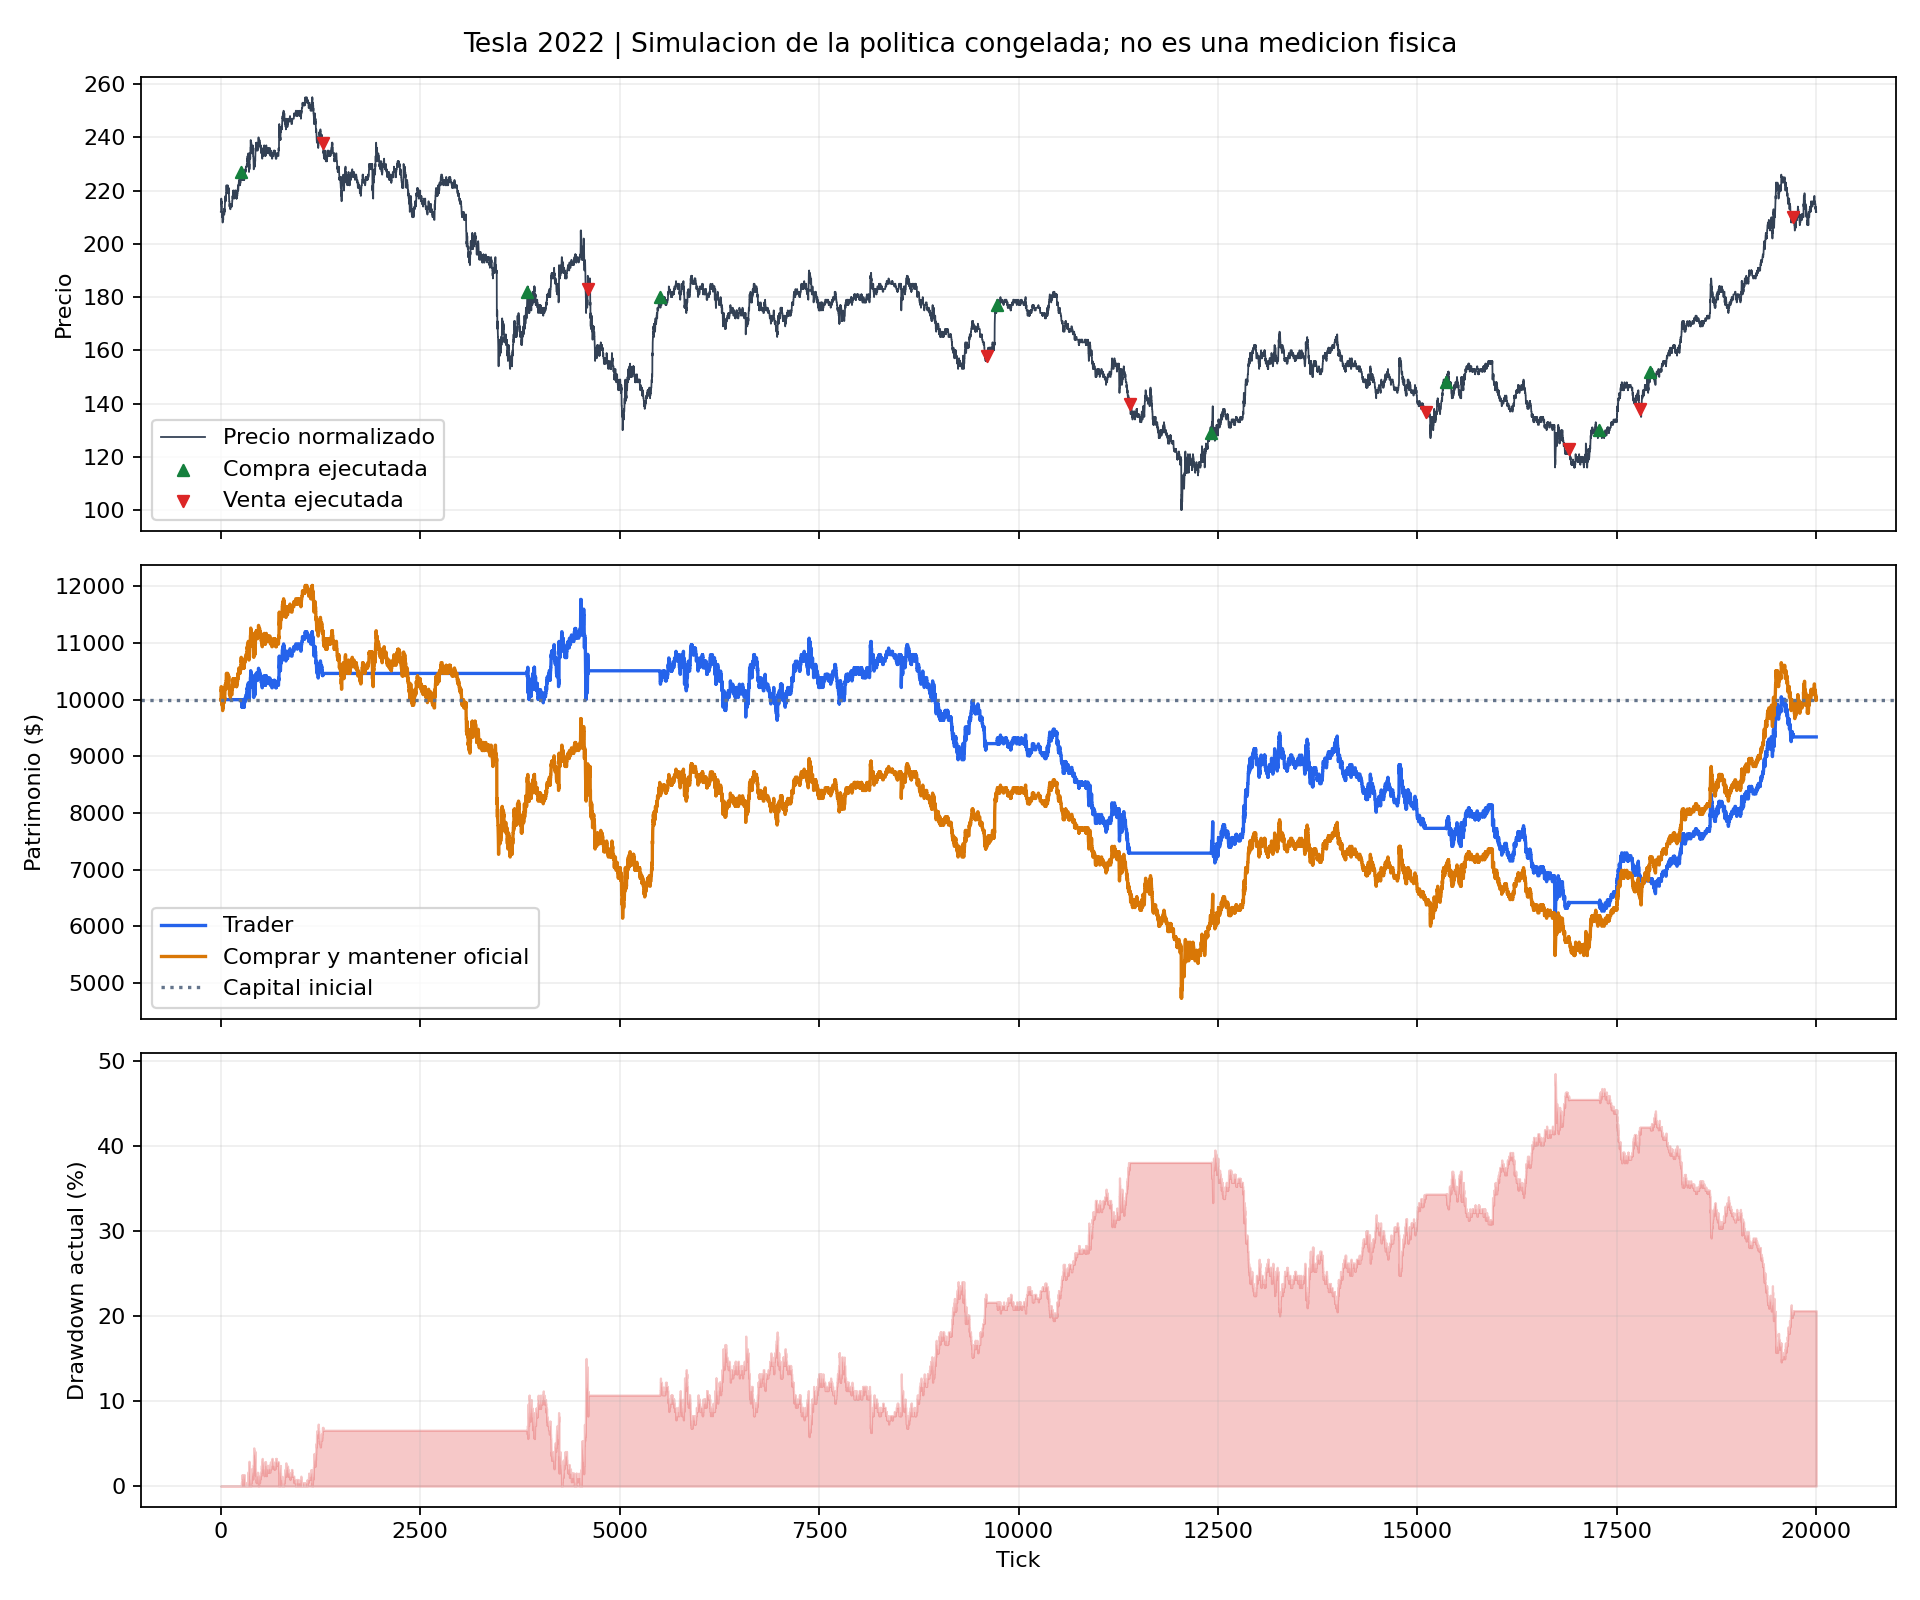
\includegraphics[width=\linewidth,height=0.70\textheight,keepaspectratio]{figuras/tesla_2022.png}\end{center}
Trader: \$9\,342; mantener: \$9\,995; ventaja: \$-653. Órdenes: 16; comisiones: \$80; drawdown máximo: 48,52\%.

Los marcadores representan ejecuciones al precio siguiente al que generó la señal. Es simulación sobre datos conocidos; no es telemetría de la placa.

\clearpage\section{Resultados de los 78 escenarios}
C/V indica compras y ventas ejecutadas. Cada escenario empieza con \$10\,000.
Los grupos y escalas comparten muestras según lo descrito en la campaña ampliada.
\small
\begin{longtable}{lrrrrr}\toprule
Serie y escala & Ticks & Trader & Mantener & C/V & DD (\%) \\\midrule\endhead
practica\_amd\_2022\_ene & 20\,000 & 10\,738 & 8\,315 & 14/13 & 42,20 \\
practica\_amd\_2022\_may & 20\,000 & 8\,540 & 9\,647 & 9/8 & 30,01 \\
practica\_apple\_2022 & 20\,000 & 14\,263 & 11\,063 & 19/19 & 38,82 \\
practica\_apple\_2023 & 20\,000 & 9\,272 & 10\,371 & 14/12 & 40,41 \\
practica\_meta\_2022 & 20\,000 & 12\,836 & 9\,695 & 5/5 & 28,13 \\
practica\_netflix\_2022 & 20\,000 & 10\,346 & 9\,179 & 15/15 & 46,72 \\
practica\_netflix\_2023 & 20\,000 & 12\,432 & 9\,170 & 14/12 & 50,55 \\
practica\_tesla\_2022 & 20\,000 & 9\,342 & 9\,995 & 8/8 & 48,52 \\
AAPL\_2019-01-02\_afin & 20\,000 & 16\,261 & 17\,585 & 5/4 & 18,04 \\
AAPL\_2020-03-23\_afin & 20\,000 & 14\,403 & 21\,385 & 4/4 & 15,14 \\
AAPL\_2021-01-04\_afin & 20\,000 & 7\,578 & 6\,927 & 16/16 & 46,77 \\
AAPL\_2022-01-03\_afin & 20\,000 & 9\,256 & 5\,996 & 11/10 & 37,84 \\
AAPL\_2023-08-01\_afin & 20\,000 & 12\,053 & 7\,070 & 8/7 & 31,15 \\
AMD\_2022-01-03\_afin & 20\,000 & 13\,517 & 5\,813 & 16/14 & 31,98 \\
AMD\_2023-05-01\_afin & 20\,000 & 17\,992 & 16\,540 & 6/4 & 31,94 \\
AMZN\_2020-03-02\_afin & 20\,000 & 15\,032 & 15\,407 & 5/5 & 22,36 \\
AMZN\_2023-01-03\_afin & 20\,000 & 18\,189 & 15\,058 & 10/8 & 18,52 \\
BA\_2020-02-03\_afin & 20\,000 & 11\,433 & 5\,417 & 4/4 & 14,46 \\
DIS\_2022-01-03\_afin & 19\,966 & 11\,903 & 6\,803 & 8/6 & 41,75 \\
GOOGL\_2021-06-01\_afin & 18\,844 & 14\,609 & 21\,470 & 8/7 & 27,80 \\
GOOGL\_2023-01-03\_afin & 20\,000 & 9\,234 & 15\,995 & 11/10 & 45,19 \\
INTC\_2022-06-01\_afin & 20\,000 & 6\,589 & 4\,925 & 8/7 & 49,20 \\
JPM\_2021-01-04\_afin & 20\,000 & 20\,698 & 21\,949 & 7/5 & 18,37 \\
JPM\_2022-01-03\_afin & 20\,000 & 7\,387 & 6\,361 & 9/8 & 44,05 \\
KO\_2019-01-02\_afin & 20\,000 & 6\,756 & 7\,658 & 6/5 & 48,62 \\
KO\_2022-06-01\_afin & 20\,000 & 7\,834 & 10\,670 & 16/16 & 50,24 \\
META\_2021-03-01\_afin & 20\,000 & 9\,564 & 17\,129 & 10/10 & 34,82 \\
META\_2022-01-03\_afin & 20\,000 & 5\,654 & 4\,847 & 4/3 & 52,05 \\
META\_2022-11-28\_afin & 20\,000 & 16\,031 & 21\,015 & 6/4 & 22,53 \\
META\_2023-06-01\_afin & 20\,000 & 11\,872 & 16\,718 & 8/7 & 25,65 \\
MSFT\_2020-02-03\_afin & 20\,000 & 13\,587 & 10\,534 & 11/10 & 40,26 \\
MSFT\_2022-01-03\_afin & 20\,000 & 10\,550 & 5\,900 & 11/9 & 26,83 \\
MSFT\_2023-01-03\_afin & 20\,000 & 13\,756 & 15\,755 & 10/9 & 24,76 \\
NFLX\_2022-01-03\_afin & 20\,000 & 8\,535 & 4\,691 & 5/3 & 36,27 \\
NFLX\_2022-04-01\_afin & 20\,000 & 5\,518 & 4\,583 & 4/3 & 48,40 \\
NVDA\_2022-01-03\_afin & 20\,000 & 12\,621 & 6\,469 & 18/16 & 31,17 \\
NVDA\_2022-09-01\_afin & 20\,000 & 8\,851 & 12\,645 & 11/10 & 42,03 \\
NVDA\_2023-01-03\_afin & 20\,000 & 16\,953 & 22\,826 & 3/2 & 16,67 \\
NVDA\_2024-01-02\_afin & 20\,000 & 16\,669 & 21\,557 & 6/4 & 16,34 \\
TSLA\_2020-06-01\_afin & 20\,000 & 19\,510 & 20\,383 & 6/4 & 24,00 \\
TSLA\_2021-01-04\_afin & 20\,000 & 9\,665 & 9\,043 & 6/6 & 45,73 \\
TSLA\_2022-01-03\_afin & 20\,000 & 9\,905 & 6\,089 & 6/5 & 33,26 \\
TSLA\_2023-01-03\_afin & 20\,000 & 15\,305 & 16\,967 & 5/5 & 18,37 \\
AAPL\_2019-01-02\_prop & 20\,000 & 10\,000 & 12\,063 & 0/0 & 0,00 \\
AAPL\_2020-03-23\_prop & 20\,000 & 13\,440 & 14\,307 & 1/0 & 9,73 \\
AAPL\_2021-01-04\_prop & 20\,000 & 10\,000 & 9\,197 & 0/0 & 0,00 \\
AAPL\_2022-01-03\_prop & 20\,000 & 10\,000 & 8\,915 & 0/0 & 0,00 \\
AAPL\_2023-08-01\_prop & 20\,000 & 10\,000 & 9\,293 & 0/0 & 0,00 \\
AMD\_2022-01-03\_prop & 20\,000 & 9\,558 & 7\,635 & 1/1 & 24,33 \\
AMD\_2023-05-01\_prop & 20\,000 & 10\,259 & 13\,073 & 1/0 & 18,91 \\
AMZN\_2020-03-02\_prop & 20\,000 & 12\,245 & 12\,245 & 1/0 & 8,53 \\
AMZN\_2023-01-03\_prop & 20\,000 & 10\,000 & 11\,503 & 0/0 & 0,00 \\
BA\_2020-02-03\_prop & 20\,000 & 9\,003 & 4\,367 & 14/12 & 35,57 \\
DIS\_2022-01-03\_prop & 19\,966 & 8\,995 & 8\,995 & 1/0 & 18,59 \\
GOOGL\_2021-06-01\_prop & 18\,844 & 10\,000 & 11\,570 & 0/0 & 0,00 \\
GOOGL\_2023-01-03\_prop & 20\,000 & 10\,000 & 11\,311 & 0/0 & 0,00 \\
INTC\_2022-06-01\_prop & 20\,000 & 10\,000 & 8\,045 & 0/0 & 0,00 \\
JPM\_2021-01-04\_prop & 20\,000 & 10\,000 & 12\,592 & 0/0 & 0,00 \\
JPM\_2022-01-03\_prop & 20\,000 & 10\,000 & 8\,683 & 0/0 & 0,00 \\
KO\_2019-01-02\_prop & 20\,000 & 10\,000 & 9\,708 & 0/0 & 0,00 \\
KO\_2022-06-01\_prop & 20\,000 & 10\,000 & 10\,115 & 0/0 & 0,00 \\
META\_2021-03-01\_prop & 20\,000 & 10\,000 & 11\,514 & 0/0 & 0,00 \\
META\_2022-01-03\_prop & 20\,000 & 10\,184 & 6\,134 & 1/0 & 3,13 \\
META\_2022-11-28\_prop & 20\,000 & 14\,322 & 15\,929 & 2/1 & 13,71 \\
META\_2023-06-01\_prop & 20\,000 & 9\,410 & 11\,264 & 1/0 & 8,10 \\
MSFT\_2020-02-03\_prop & 20\,000 & 12\,035 & 10\,253 & 1/0 & 11,39 \\
MSFT\_2022-01-03\_prop & 20\,000 & 10\,000 & 8\,669 & 0/0 & 0,00 \\
MSFT\_2023-01-03\_prop & 20\,000 & 10\,000 & 11\,480 & 0/0 & 0,00 \\
NFLX\_2022-01-03\_prop & 20\,000 & 11\,568 & 5\,978 & 3/1 & 13,72 \\
NFLX\_2022-04-01\_prop & 20\,000 & 5\,863 & 4\,747 & 3/2 & 45,34 \\
NVDA\_2022-01-03\_prop & 20\,000 & 11\,809 & 8\,155 & 2/1 & 11,47 \\
NVDA\_2022-09-01\_prop & 20\,000 & 10\,793 & 11\,271 & 1/0 & 2,69 \\
NVDA\_2023-01-03\_prop & 20\,000 & 16\,043 & 17\,447 & 1/0 & 11,03 \\
NVDA\_2024-01-02\_prop & 20\,000 & 11\,387 & 18\,003 & 1/0 & 12,73 \\
TSLA\_2020-06-01\_prop & 20\,000 & 14\,385 & 17\,366 & 3/2 & 17,79 \\
TSLA\_2021-01-04\_prop & 20\,000 & 11\,289 & 9\,456 & 2/1 & 15,96 \\
TSLA\_2022-01-03\_prop & 20\,000 & 9\,885 & 7\,412 & 1/0 & 24,41 \\
TSLA\_2023-01-03\_prop & 20\,000 & 14\,967 & 15\,251 & 1/1 & 13,35 \\
\bottomrule\end{longtable}\normalsize

\end{document}
